\documentclass[11pt,a4paper]{article}
\usepackage[T1]{fontenc}
\usepackage[utf8]{inputenc}
\usepackage{lmodern,microtype}
\usepackage[margin=25mm]{geometry}
\usepackage{amsmath,amssymb,amsthm,mathtools}
\usepackage{booktabs,array}
\usepackage{placeins}
\usepackage[dvipsnames]{xcolor}
\usepackage{enumitem}
\usepackage{algorithm}
\usepackage{algpseudocode}
\usepackage{tikz}
\usetikzlibrary{arrows.meta,positioning,calc,fit,shapes.misc}
\usepackage{pgfplots}
\pgfplotsset{compat=1.17}
\usepackage{hyperref}
\hypersetup{colorlinks=true,linkcolor=NavyBlue,citecolor=ForestGreen,urlcolor=NavyBlue,
  pdftitle={Two-round subsampled randomized Hadamard transforms},
  pdfauthor={Diar Heidary}}
\setlength{\emergencystretch}{2em}
\allowdisplaybreaks
\setlist{itemsep=0.2em,topsep=0.3em}

\newtheorem{theorem}{Theorem}[section]
\newtheorem{lemma}[theorem]{Lemma}
\newtheorem{proposition}[theorem]{Proposition}
\newtheorem{corollary}[theorem]{Corollary}
\newtheorem{imported}[theorem]{Imported theorem}
\newtheorem{conjecture}[theorem]{Conjecture}
\newtheorem*{theoremA}{Theorem A (canonical prescription)}
\newtheorem*{theoremB}{Theorem B (direct selector)}
\newtheorem*{theoremC}{Theorem C (whole-sketch Nystr\"om energy)}
\newtheorem*{theoremD}{Theorem D (RP-selected frames)}
\newtheorem*{theoremE}{Theorem E (fresh-row drift)}
\theoremstyle{definition}
\newtheorem{definition}[theorem]{Definition}
\theoremstyle{remark}
\newtheorem{remark}[theorem]{Remark}
\numberwithin{equation}{section}

\newcommand{\E}{\mathbb E}
\newcommand{\Prob}{\mathbb P}
\newcommand{\R}{\mathbb R}
\newcommand{\C}{\mathbb C}
\newcommand{\tr}{\operatorname{tr}}
\newcommand{\Diag}{\operatorname{Diag}}
\newcommand{\diag}{\operatorname{diag}}
\newcommand{\Var}{\operatorname{Var}}
\newcommand{\range}{\operatorname{range}}
\newcommand{\Bin}{\operatorname{Bin}}
\newcommand{\eps}{\varepsilon}
\newcommand{\norm}[1]{\lVert#1\rVert}
\newcommand{\Nys}{\mathcal N}
\newcommand{\cT}{\mathcal T}
\newcommand{\Cert}{\operatorname{Cert}}
\newcommand{\Rex}{\mathcal R}

\title{Two-round subsampled randomized Hadamard transforms:\\
canonical prescriptions, whole-sketch Nystr\"om energy,\\
and adaptive frames}
\author{Diar Heidary}
\date{29 September 2026}

% Shared manuscript typography. Keep this file beside the manuscript folders.
\usepackage{needspace}
\usepackage{etoolbox}
\linespread{1.08}
\setlength{\parskip}{0.38em plus 0.08em minus 0.05em}
\setlength{\parindent}{1.25em}
\setlength{\emergencystretch}{2em}
\setlist{itemsep=4pt,topsep=6pt,parsep=2pt}
\renewcommand{\arraystretch}{1.16}
\setlength{\tabcolsep}{6pt}
\AtBeginDocument{%
  \setlength{\abovedisplayskip}{10pt plus 2pt minus 2pt}%
  \setlength{\belowdisplayskip}{10pt plus 2pt minus 2pt}%
  \setlength{\abovedisplayshortskip}{5pt plus 2pt}%
  \setlength{\belowdisplayshortskip}{8pt plus 2pt minus 2pt}%
}
\makeatletter
\def\th@plain{%
  \thm@preskip=10pt plus 2pt minus 2pt
  \thm@postskip=10pt plus 2pt minus 2pt
  \itshape
}
\def\th@definition{%
  \thm@preskip=10pt plus 2pt minus 2pt
  \thm@postskip=10pt plus 2pt minus 2pt
  \normalfont
}
\def\th@remark{%
  \thm@headfont{\itshape}%
  \thm@preskip=9pt plus 2pt minus 2pt
  \thm@postskip=9pt plus 2pt minus 2pt
  \normalfont
}
\makeatother
\AtBeginEnvironment{proof}{\Needspace{4\baselineskip}}
\widowpenalty=10000
\clubpenalty=10000
\displaywidowpenalty=10000
\raggedbottom

\begin{document}
\maketitle

\begin{abstract}
Two rounds of sign randomization and unitary mixing admit smaller certified
subspace embeddings when the sampling density is retained throughout the
moment argument. Starting from a previously established row-factor estimate
$\Lambda_q$, we prove the explicit prescription
\[
 q=\left\lceil\log_4\frac{6d}{5\delta}\right\rceil,
 \qquad M=\min\{n,\lceil20\Lambda_q/\varepsilon^2\rceil\}.
\]
It reduces the earlier sufficient coefficient $72$ to $20$, without changing
the sketch distribution; direct evaluation of the resulting moment bound
can reduce the certified width further. Independently of the imported
operator estimates, we derive exact fourth-moment identities for one
without-replacement sketch and the Nystr\"om bound
$\E\|K-\mathcal N_K(S^*)\|_F^2\le
2(1-M/n)(\tr K)^2/M$ for real flat transforms. These identities support
nonadaptive trace and diagonal estimators. We also transfer fixed-frame
guarantees to a restricted form of sketch-dependent frame selection using
the classical comparison between adaptive and volume sampling.
\end{abstract}

\tableofcontents

%======================================================================
\section{Introduction and main results}\label{sec:intro}

A structured embedding is useful only when its row budget is explicit.
For the two-round transform studied here, previous operator estimates
already give a dimension term plus a quadratic confidence term. This paper
asks a narrower quantitative question: how much of the stated row budget
comes from the operator estimate, and how much comes from the final scalar
calibration?

The main answer is that retaining the actual sampling density and the exact
Bernoulli-to-fixed-size comparison reduces one sufficient coefficient from
$72$ to $20$. The sketch and the imported row-factor estimate are unchanged.
A separate fourth-moment calculation describes what one entire sketch can
do for Nystr\"om approximation. Keeping these two arguments separate makes
their assumptions and their respective strengths explicit.

\subsection{The model}\label{sec:model}
Let $A,B\in\C^{n\times n}$ be unitary, with coherences
\begin{equation}\label{eq:coherence}
 \alpha=n\max_{j,a}|A_{ja}|^2,\qquad \beta=n\max_{a,i}|B_{ai}|^2 .
\end{equation}
Both are at least one, and both equal one exactly when the matrix is
\emph{flat}, $|A_{ja}|^2=1/n$; the normalized Walsh--Hadamard matrix
$H_n$ ($n$ a power of two) and the normalized discrete Fourier matrix are
flat. Let $D_x,D_y$ be diagonal matrices of unbiased signs, the two
families being independent, and let $\cT\subseteq[n]$ be a uniform
$M$-element subset, independent of the signs. With $R_\cT$ the coordinate
restriction to $\cT$, the \emph{two-round sketch} is
\begin{equation}\label{eq:sketch}
 Q=AD_yBD_x,\qquad S=\sqrt{n/M}\,R_\cT Q\in\C^{M\times n}.
\end{equation}
For a fixed isometry $U\in\C^{n\times d}$ ($U^*U=I_d$) the Gram error is
\[
 E_\cT=U^*S^*SU-I_d=\frac nM\sum_{j\in\cT}w_jw_j^*-I_d,
 \qquad w_j^*=e_j^*QU,\qquad \sum_{j=1}^nw_jw_j^*=I_d .
\]
The event $\norm{E_\cT}\le\eps$ is the $(1\pm\eps)$ subspace-embedding
event for $\range U$. The classical (one-round) SRHT of
Ailon--Chazelle and Tropp~\cite{AilonChazelle,TroppSRHT} is the case
$B=I$ (then $D_yD_x$ is a single sign diagonal). Throughout, $1\le d\le n$
and $q\ge1$ is an integer; the even trace moment $\E\tr E_\cT^{2q}$ is the
basic object.

Put
\begin{equation}\label{eq:allowances}
\begin{gathered}
 a_q=\alpha q(2q+1),\qquad b_q=\beta(d+8q^2)+\alpha q(2q-1),\\
 D_q=a_q+b_q=\beta d+(8\beta+4\alpha)q^2,\qquad
 \Lambda_q=\bigl(\sqrt{a_q}+\sqrt{2b_q}\bigr)^2 .
\end{gathered}
\end{equation}
For flat transforms $D_q=d+12q^2$. Always
\begin{equation}\label{eq:LambdaD}
 D_q\le\Lambda_q\le3D_q,
\end{equation}
since $\Lambda_q=a_q+2b_q+2\sqrt{2a_qb_q}\ge a_q+b_q$ and, by
Cauchy--Schwarz, $(\sqrt{a_q}\cdot1+\sqrt{b_q}\cdot\sqrt2)^2\le3(a_q+b_q)$.
For sampling we write
\begin{equation}\label{eq:rho-atom}
 \rho=\frac Mn,\qquad
 p_{n,M}=\Prob\{\Bin(n-1,\rho)=M\},\qquad
 \lambda_{n,M}=\frac{n-M}{M(n-1)}\quad(n\ge2).
\end{equation}

\subsection{Main results}\label{sec:main}
The first result is the canonical sampling prescription. It rests on the
retained row-factor estimate and the graded multiplication-operator moment
identity, which we import (Section~\ref{sec:imported}).

\begin{theoremA}
Let $0<\eps<1$ and $q\ge1$. For every integer $M$ with
$\min\{n,\lceil20\Lambda_q/\eps^2\rceil\}\le M\le n$ and every fixed isometry
$U$,
\[
 \Prob\{\norm{E_\cT}>\eps\}\le\tfrac65\,d\,4^{-q}.
\]
Consequently, for $0<\delta<1$,
\begin{equation}\label{eq:canonical}
 \boxed{\;q_*=\Bigl\lceil\log_4\frac{6d}{5\delta}\Bigr\rceil,\qquad
 M=\min\bigl\{n,\lceil20\Lambda_{q_*}/\eps^2\rceil\bigr\}\;}
\end{equation}
gives $\Prob\{\norm{E_\cT}>\eps\}\le\delta$. Each sign family may be only
$\min(n,4q)$-wise independent, provided the two families and $\cT$ are
mutually independent. Since $\Lambda_q\le3D_q$, the coherence-only
prescription $M=\min\{n,\lceil60D_{q_*}/\eps^2\rceil\}$ has the same
guarantee.
\end{theoremA}

The constant $20$ calibrates the \emph{exact} moment root
(Theorem~\ref{thm:exactroot}); $72\Lambda_q$ and $216D_q$ calibrate a crude
relaxation of it. Section~\ref{sec:chain} proves the ordering
$216D_q\ge72\Lambda_q>60D_q\ge20\Lambda_q$ and explains where each factor
comes from (Figure~\ref{fig:chain}).

\begin{theoremB}
For each prescribed pair $(q,M)$ with $q\ge1$ and $1\le M<n$,
the explicit quantity
\[
 \Cert(q,M)=d\,[\Rex_q(M)/\eps]^{2q}
\]
from Theorem~\ref{thm:exactroot} bounds the embedding failure probability.
Algorithm~\ref{alg:selector} returns only a pair whose certificate is at
most $\delta$, or the exact sketch $M=n$. Its guarantee uses
$\min(n,4q)$-wise independence at the returned order.

The ideal minimum over the searched orders is no larger than the canonical
prescription if $q_{\max}\ge q_*$. A bisection implementation is a search
heuristic, rather than a proof of that minimum. In the four examples
$d=10,10^2,10^3,10^4$ at $n=2^{30}$, $\eps=1/2$, $\delta=0.01$, the
checked returned widths are respectively
\[
 58\,406,\quad125\,760,\quad346\,325,\quad1\,423\,405.
\]
They are smaller than the canonical widths
$102\,608$, $157\,664$, $427\,412$, and $2\,192\,958$.
\end{theoremB}

\begin{theoremD}
Fix an isometry $V\in\C^{N\times k}$ and, for each $k$-subset $J\subseteq[N]$,
a target isometry $U_J$, before the sketch is drawn. After drawing $S$, choose
any positive definite $C(S)$ and run $k$ steps of randomly pivoted Cholesky
on $VC(S)V^*$; release the unordered pivot set $J$. If
$\Gamma_{C(S)}\le\overline\Gamma$ almost surely, where
$\Gamma_C=k!\det C/\prod_{j<k}\tau_j(C)\in[1,k!]$, then the selected frame
satisfies $\Prob\{\norm{U_J^*S^*SU_J-I_d}>\eps\}\le\delta$ with the
prescription~\eqref{eq:canonical} at confidence $\delta/\overline\Gamma$.
For $k=2$ the allowance $\delta/2$ always suffices and beats the
second-moment allowance $8\delta^2/9$ for every $\delta<9/16$.
\end{theoremD}

\begin{theoremC}
Let $A$ be flat and $B$ unitary, let the sign families be four-wise
independent, and let $K\succeq0$. With
$\Nys_K(S^*)=KS^*(SKS^*)^\dagger SK$,
\[
 \E\norm{K-\Nys_K(S^*)}_F^2
 \le\lambda_{n,M}\bigl[(\tr K)^2+\norm K_F^2\bigr].
\]
If $K$ is real and $A,B$ are real flat orthogonal matrices (e.g.\ $A=B=H_n$),
the Gram-error energy has the exact value
$\lambda_{n,M}[(1-\tfrac2n)(\tr K)^2+(1-\tfrac4n)\norm K_F^2+\tfrac4n\sum_iK_{ii}^2]$
and
\[
 \boxed{\E\norm{K-\Nys_K(S^*)}_F^2\le\frac2M\Bigl(1-\frac Mn\Bigr)(\tr K)^2.}
\]
The one-round real flat law ($B=I$) has exact Gram-error energy
$\lambda_{n,M}[(\tr K)^2+\norm K_F^2-2\sum_iK_{ii}^2]$ and satisfies the same
boxed bound.
\end{theoremC}

The bound is rank-blind: it is an approximate-matrix-multiplication
variance~\cite{DKM} for the product $K^{1/2}\cdot K^{1/2}$, not a
relative-error low-rank guarantee. Its virtue is that it counts the actual
$M$ rows of one sketch with shared signs and reaches zero at $M=n$.
It yields an $O(1/\eps)$-query trace estimator and an $O(1/\eps)$-query
diagonal estimator (Corollaries~\ref{cor:trace} and~\ref{cor:diag}).

\begin{theoremE}
For flat $A$, a fixed row $j$ of a freshly drawn $Q$, and
$z=\sqrt n\,Q^*e_j$, every PSD $R_0\ne0$ satisfies
$\E(\tr R_0-\tr R_1)\ge\tr(R_0^2)/(\kappa_0\tr R_0)$ for the Nystr\"om update
$R_1=R_0-R_0z(z^*R_0z)^\dagger z^*R_0$, where
$\kappa_0=e^{2-\gamma}/2=2.0743\ldots$, with $\gamma$ Euler's constant. Only one Khintchine factor occurs,
not one per transform, and $\kappa_0$ equals the constant of an i.i.d.\
Rademacher probe.
\end{theoremE}

Section~\ref{sec:sketchedrp} places the canonical prescription inside the
path-local embedding framework for sketched randomly pivoted Cholesky
developed in \emph{RPCholesky under approximate and sketched pivot
probabilities}~\cite{RobustRP}.

\subsection{Contributions and relation to earlier work}

\paragraph{The embedding order is an earlier result.}
The one-round SRHT and its subspace-embedding analysis are established
tools~\cite{AilonChazelle,DMMS,TroppSRHT,BoutsidisGittens}.
The present two-round Walsh distribution is the rerandomized transform in
Amsel et al.~\cite[Definition~5.3 and Problem~5.6]{Amsel}.
Yang~\cite[Theorem~1]{Yang} proves the prescribed constant-failure width
$M=\min\{n,\lceil C d/\eps^2\rceil\}$ for fixed real frames under this exact two-Walsh law.
The earlier repository paper~\cite{SRHT2R} gives a different argument with
allowance $d+27q^3$; the graded framework~\cite[Theorem~10.1]{V11}
gives the quadratic allowance $D_q$ for arbitrary coherent unitary pairs.
We claim neither the first two-round embedding theorem nor a new optimal
asymptotic row order at constant confidence.

\paragraph{What the present calibration adds.}
The retained row-factor analysis~\cite[Theorem~4.1]{HY} supplies
$\Lambda_q$ and the density-sensitive Bernoulli moment bound used here.
The exact barycenter coupling is also already proved in that analysis and
in the graded framework. Their stated prescriptions use the relaxations
$c^{-1}\le2$ and $1-\rho\le1$. We instead retain
$c=1-p_{n,M}$ and $\rho=M/n$ together. An elementary binomial-atom estimate
then gives the sufficient coefficient $20\Lambda_q$, or $60D_q$, in place
of $72\Lambda_q$, or $216D_q$. This is an improvement to these particular
sufficient conditions; it does not establish that the constants are
optimal, or that they improve every earlier analysis of the Walsh law.
Searching the explicit bound over $(q,M)$ recovers further scalar slack.
The quadratic confidence allowance remains unchanged.

\paragraph{Whole-sketch consequences and inherited ideas.}
The finite-population fourth-moment identities in
Section~\ref{sec:nystrom} apply to all rows of one actual sketch, which
share both sign diagonals. They yield a rank-blind Nystr\"om estimate and
structured-sketch versions of the sketch-and-correct ideas in
Hutch++~\cite{Hutchpp} and Diag++~\cite{BN}; the $O(1/\eps)$ query order
and the variance-reduction principle are earlier results. Approximate
matrix multiplication provides the relevant error scale~\cite{DKM}.
In particular, Nystr\"om++~\cite{Nystrompp} already combines a Nystr\"om
approximation with independent residual probes in one pass. Our trace
estimator instantiates that idea with the present without-replacement
structured sketch and its explicit second-moment bound.
SRHT-based Nystr\"om approximation itself is also established
work~\cite{BBGL}, including block constructions for distributed systems.

The adaptive-frame argument specializes the classical adaptive-to-volume
sampling comparison of Deshpande and Vempala~\cite[Proposition~7]{DV}.
It has the same fixed-range limitation as the gate used in the repository
SparseStack companion~\cite{SparseCompanion}. Its contribution here is the
explicit SRHT budget obtained by combining that comparison with the
canonical prescription. The fresh-row drift is a Khintchine-based
specialization of the product-probe argument~\cite{PP}, with the same
constant as a Rademacher probe.

\paragraph{Other sampling comparisons.}
Gross and Nesme~\cite{GrossNesme} establish the classical comparison
between sampling with and without replacement for a finite matrix
collection. Our auxiliary comparison is between Bernoulli sampling and a
fixed-size subset, with a centered conditional barycenter; these are
different sampling laws. The general algorithmic role of structured
dimension reduction, including weaker injectivity guarantees, is developed
by Cama\~no et al.~\cite{CEMT}. No injectivity result is substituted for the
two-sided subspace embedding required here.

\subsection{Roadmap}
Figure~\ref{fig:roadmap} shows the logical structure. The imported
operator estimates are used only through Imported
Theorem~\ref{imp:bernoulli}. Sections~\ref{sec:exactroot}--\ref{sec:selector}
turn it into prescriptions; Section~\ref{sec:gate} makes the frame adaptive;
Sections~\ref{sec:nystrom}--\ref{sec:drift} are independent of the moment
machinery and use only fourth moments and Khintchine's inequality;
Section~\ref{sec:sketchedrp} connects to sketched pivoting;
Section~\ref{sec:numerics} contains all numerical tables.

\begin{figure}[t]
\centering
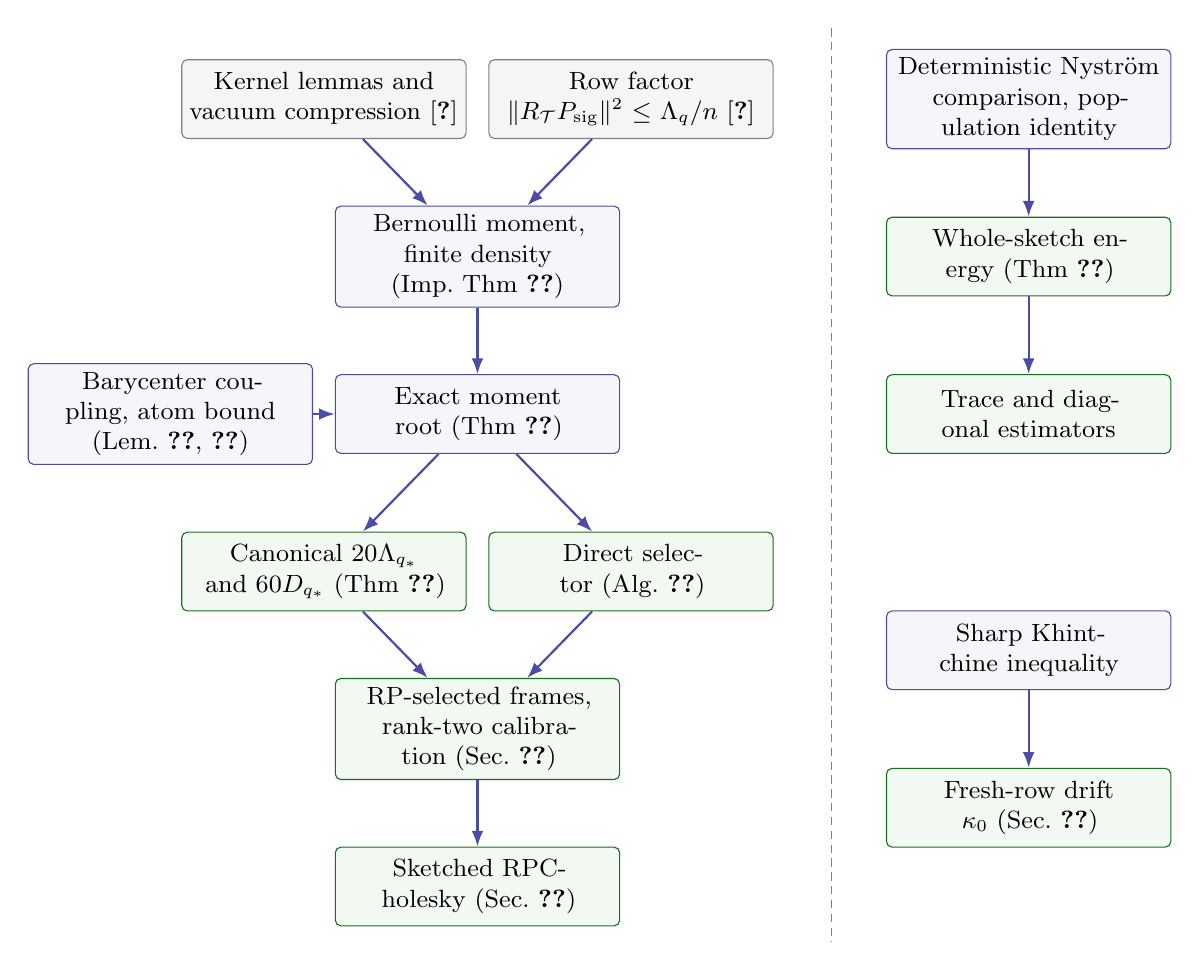
\begin{tikzpicture}[
  box/.style={draw=NavyBlue!70,fill=NavyBlue!4,rounded corners=2pt,align=center,
     font=\small,inner sep=3pt,text width=34mm,minimum height=10mm},
  imp/.style={box,draw=Gray,fill=Gray!8},
  res/.style={box,draw=ForestGreen!80!black,fill=ForestGreen!6},
  arr/.style={-{Latex[length=2mm]},thick,draw=NavyBlue!70}]
\node[imp] (v11) at (1.95,0) {Kernel lemmas and vacuum compression~\cite{V11}};
\node[imp] (hy) at (5.85,0) {Row factor $\norm{R_\cT P_{\rm sig}}^2\le\Lambda_q/n$~\cite{HY}};
\node[box] (bern) at (3.9,-2) {Bernoulli moment, finite density (Imp.~Thm~\ref{imp:bernoulli})};
\node[box] (coup) at (0,-4) {Barycenter coupling, atom bound (Lem.~\ref{lem:coupling}, \ref{lem:atom})};
\node[box] (root) at (3.9,-4) {Exact moment root (Thm~\ref{thm:exactroot})};
\node[res] (canon) at (1.95,-6) {Canonical $20\Lambda_{q_*}$ and $60D_{q_*}$ (Thm~\ref{thm:20})};
\node[res] (sel) at (5.85,-6) {Direct selector (Alg.~\ref{alg:selector})};
\node[res] (gate) at (3.9,-8) {RP-selected frames, rank-two calibration (Sec.~\ref{sec:gate})};
\node[res] (skrp) at (3.9,-10) {Sketched RPCholesky (Sec.~\ref{sec:sketchedrp})};
\node[box] (det) at (10.9,0) {Deterministic Nystr\"om comparison, population identity};
\node[res] (whole) at (10.9,-2) {Whole-sketch energy (Thm~\ref{thm:whole})};
\node[res] (est) at (10.9,-4) {Trace and diagonal estimators};
\node[box] (kh) at (10.9,-7) {Sharp Khintchine inequality};
\node[res] (drift) at (10.9,-9) {Fresh-row drift $\kappa_0$ (Sec.~\ref{sec:drift})};
\draw[densely dashed,Gray] (8.4,0.9)--(8.4,-10.7);
\draw[arr] (v11)--(bern); \draw[arr] (hy)--(bern);
\draw[arr] (bern)--(root); \draw[arr] (coup)--(root);
\draw[arr] (root)--(canon); \draw[arr] (root)--(sel);
\draw[arr] (canon)--(gate); \draw[arr] (sel)--(gate);
\draw[arr] (gate)--(skrp);
\draw[arr] (det)--(whole); \draw[arr] (whole)--(est);
\draw[arr] (kh)--(drift);
\end{tikzpicture}
\caption{Roadmap. Grey: imported results. Green: results of this paper.
The right column uses only fourth moments and Khintchine's inequality.}
\label{fig:roadmap}
\end{figure}

%======================================================================
\section{Imported results and limited independence}\label{sec:imported}

The embedding prescriptions are conditional on the following previously
proved estimate. We state its complete hypotheses so that readers can use
the scalar argument without reconstructing the underlying operator
notation. Its proof is in the repository row-factor paper~\cite{HY},
with the coefficient kernels supplied by the graded framework~\cite{V11}.
Neither this section nor the numerical checks below constitute a new
verification of all those imported kernels.

Let
$(\eta_j)_{j\le n}$ be independent Bernoulli$(\rho)$ selectors, independent of
the signs, $0<\rho<1$, $m=\rho n$, and
\[
 E_\rho=\rho^{-1}W^*\Diag(\eta)W-I_d=\sum_j(\eta_j/\rho-1)w_jw_j^*,
 \qquad W=QU .
\]

\begin{imported}[Retained row factor and Bernoulli moments; \cite{HY}, building on~\cite{V11}]
\label{imp:bernoulli}
Under fully independent signs and selectors, for every integer $q\ge1$,
\begin{equation}\label{eq:bernoulli}
 \E\tr E_\rho^{2q}\le d\left[2\sqrt{\frac{(1-\rho)\Lambda_q}{m}}
 +|1-2\rho|\frac{\Lambda_q}{m}\right]^{2q}.
\end{equation}
\end{imported}

\begin{remark}[Provenance of~\eqref{eq:bernoulli}]
In~\cite{V11} the error $E_\rho$ is represented as a multiplication operator
on the finite product space of sign monomials and selector monomials, and
$\E\tr E_\rho^{2q}=\sum_{a\le d}\norm{M_{\rm cut}^q(e_a\otimes\Omega)}^2$
exactly, where $M_{\rm cut}$ is the multiplication operator compressed to
sign grades at most $2q$ and selector grade at most $q$ (one multiplication
moves each sign grade by at most two and the selector grade by at most one).
In the normalized basis of a selector site, multiplication by $\eta/\rho-1$ is
$\bigl(\begin{smallmatrix}0&\sigma\\\sigma&\tau\end{smallmatrix}\bigr)$ with
$\sigma=\sqrt{(1-\rho)/\rho}$, $\tau=(1-2\rho)/\rho$, and the positive-selector
lemma of~\cite{V11} gives $\norm{M_{\rm cut}}\le2\sigma\sqrt{L_q}+|\tau|L_q$,
where $L_q$ is the largest norm of a sum of at most $q$ compressed positive
row effects. The retained row-factor theorem of~\cite{HY} bounds the row map
before forming its Gram,
$\norm{R_\cT P_{\rm sig}}^2\le\Lambda_q/n$ for $|\cT|\le q$, so
$L_q\le\min\{1,\Lambda_q/n\}$; substituting gives~\eqref{eq:bernoulli}. That
theorem uses the joint-creation, mixed-channel and collective
double-annihilation kernel bounds of~\cite{V11}. The earlier bound
$L_q\le9D_q/n$ of~\cite{V11} gives the same statement with $\Lambda_q$
replaced by $9D_q$.
\end{remark}

\begin{lemma}[Limited independence]\label{lem:limited}
Every entry of $E_\cT$ and of $E_\rho$ is a polynomial of degree at most two in
each sign family. Hence $\E\tr E_\cT^{2q}$ is unchanged if each sign family is
only $\min(n,4q)$-wise independent and unbiased, provided the two families and
the subset (or the selectors) are mutually independent.
\end{lemma}
\begin{proof}
$w_jw_j^*$ has entries $\sum_{a,b,i,l}A_{ja}\overline{A_{jb}}B_{ai}\overline{B_{bl}}
y_ay_bx_ix_lU_{i\cdot}\overline{U_{l\cdot}}$, of degree two in $x$ and in $y$.
Expanding $\tr E_\cT^{2q}$ produces a linear combination of monomials, each
involving at most $4q$ distinct coordinates of either family. The
expectation of such a monomial depends only on the joint law of at most
$\min(n,4q)$ coordinates of each family, which is the uniform law on signs
under $\min(n,4q)$-wise independence. Conditioning on the subset, which is
independent of the signs, completes the proof.
\end{proof}

%======================================================================
\section{The exact moment root}\label{sec:exactroot}

\subsection{From Bernoulli to fixed-size sampling}
Fix Hermitian matrices $H_1,\dots,H_n$ and $1\le M<n$, $\rho=M/n$. For a
Bernoulli$(\rho)$ subset $\mathcal B$ and a uniform $M$-subset $\cT$ put
\[
 Z_{\mathcal B}=\sum_j(\mathbf 1_{j\in\mathcal B}-\rho)H_j,\qquad
 Z_\cT=\sum_j(\mathbf 1_{j\in\cT}-\rho)H_j .
\]

\begin{lemma}[Exact barycenter coupling]\label{lem:coupling}
There is a coupling of $\mathcal B$ and $\cT$ such that
\[
 \E[Z_{\mathcal B}\mid\cT]=c\,Z_\cT,\qquad c=1-p_{n,M}\ge\tfrac12 .
\]
Consequently, for every integer $q\ge1$,
$\E\tr Z_\cT^{2q}\le c^{-2q}\,\E\tr Z_{\mathcal B}^{2q}$.
\end{lemma}
\begin{proof}
Draw $\mathcal B$, with size $K\sim\Bin(n,\rho)$. If $K>M$ delete $K-M$
uniformly chosen elements; if $K<M$ add $M-K$ uniformly chosen missing
elements. By symmetry $\cT$ is a uniform $M$-subset (independent of $K$), and
conditionally on $\cT$ the law of $\mathcal B$ is invariant under
permutations fixing $\cT$. Hence $\Prob(j\in\mathcal B\mid\cT)$ takes one
value $\theta_1$ for $j\in\cT$ and one value $\theta_0$ for $j\notin\cT$. An
element of $\cT$ is missing from $\mathcal B$ only if it was added, and an
element outside $\cT$ lies in $\mathcal B$ only if it was deleted, so with
$a=\E(K-M)_+=\E(M-K)_+$ (equal because $\E K=M$),
\[
 \theta_1=1-\frac aM,\qquad\theta_0=\frac a{n-M}.
\]
With $v=n\rho(1-\rho)=M(1-\rho)=\rho(n-M)$ we get
$\theta_1-\rho=(1-\rho)(1-a/v)$ and $\theta_0-\rho=-\rho(1-a/v)$, so
$\E[\mathbf 1_{j\in\mathcal B}-\rho\mid\cT]=(1-a/v)(\mathbf 1_{j\in\cT}-\rho)$
and $\E[Z_{\mathcal B}\mid\cT]=(1-a/v)Z_\cT$.

Let $Y\sim\Bin(n-1,\rho)$ and write $K=Y+\xi$ with an independent
Bernoulli$(\rho)$ variable $\xi$. The identity $k\binom nk=n\binom{n-1}{k-1}$
gives $\E[K\mathbf 1_{K\ge M+1}]=n\rho\Prob(Y\ge M)=M\Prob(Y\ge M)$, and
$\Prob(K\ge M+1)=\Prob(Y\ge M+1)+\rho\Prob(Y=M)$. Therefore
\[
 a=\E[K\mathbf 1_{K\ge M+1}]-M\Prob(K\ge M+1)=M(1-\rho)\Prob(Y=M)=v\,p_{n,M},
\]
so $1-a/v=1-p_{n,M}=c$. The atoms $\Prob(Y=M)$ and $\Prob(Y=M-1)$ have ratio
$\frac{n-M}{M}\cdot\frac\rho{1-\rho}=1$, so each is at most $1/2$ and
$c\ge1/2$.

Finally $Z\mapsto\tr Z^{2q}=\norm Z_{S_{2q}}^{2q}$ is convex on Hermitian
matrices, and conditional Jensen gives
$\E\tr Z_{\mathcal B}^{2q}\ge\E\tr(\E[Z_{\mathcal B}\mid\cT])^{2q}
=c^{2q}\E\tr Z_\cT^{2q}$.
\end{proof}

\begin{lemma}[Binomial atom]\label{lem:atom}
For $1\le M<n$, $\rho=M/n$ and $v=M(1-\rho)$,
\[
 p_{n,M}=\Prob\{\Bin(n-1,\rho)=M\}=\Prob\{\Bin(n,\rho)=M\}
 \le\min\Bigl\{\frac12,\ \sqrt{\frac{\pi}{8v}}\Bigr\}.
\]
\end{lemma}
\begin{proof}
The equality follows from $\binom{n-1}M=(1-\rho)\binom nM$, and the bound
$1/2$ was shown in Lemma~\ref{lem:coupling}. By Fourier inversion,
\[
 \Prob\{\Bin(n,\rho)=M\}
 =\frac1{2\pi}\int_{-\pi}^{\pi}(1-\rho+\rho e^{it})^ne^{-iMt}\,dt
 \le\frac1{2\pi}\int_{-\pi}^{\pi}|1-\rho+\rho e^{it}|^n\,dt .
\]
Now $|1-\rho+\rho e^{it}|^2=1-4\rho(1-\rho)\sin^2(t/2)\le
\exp\{-4\rho(1-\rho)\sin^2(t/2)\}$, so the integrand is at most
$\exp\{-2v\sin^2(t/2)\}$. On $[-\pi,\pi]$ concavity of the sine gives
$|\sin(t/2)|\ge|t|/\pi$. Extending the Gaussian integral to $\R$,
\[
 p_{n,M}\le\frac1{2\pi}\int_\R e^{-2vt^2/\pi^2}\,dt
 =\frac1{2\pi}\cdot\pi\sqrt{\frac{\pi}{2v}}=\sqrt{\frac\pi{8v}} .\qedhere
\]
\end{proof}

\subsection{The root}
\begin{theorem}[Exact moment root]\label{thm:exactroot}
Let $1\le M<n$ and $\rho=M/n$. For every integer $q\ge1$ and every fixed
isometry $U$,
\begin{equation}\label{eq:exactroot}
 \E\tr E_\cT^{2q}\le d\,\Rex_q(M)^{2q},\qquad
 \Rex_q(M)=\frac{2\sqrt{(1-\rho)\Lambda_q/M}+|1-2\rho|\,\Lambda_q/M}{1-p_{n,M}} .
\end{equation}
In particular, for every $\eps>0$,
\begin{equation}\label{eq:cert}
 \Prob\{\norm{E_\cT}>\eps\}\le\Cert(q,M):=d\left(\frac{\Rex_q(M)}{\eps}\right)^{2q}.
\end{equation}
Both statements hold under $\min(n,4q)$-wise independent signs. For $M=n$ the
error vanishes identically.
\end{theorem}
\begin{proof}
Condition on the signs and apply Lemma~\ref{lem:coupling} to $H_j=w_jw_j^*$.
Since $\sum_jw_jw_j^*=I_d$, we have $E_\cT=\rho^{-1}Z_\cT$ and
$E_\rho=\rho^{-1}Z_{\mathcal B}$ with $m=\rho n=M$. Averaging over the signs,
$\E\tr E_\cT^{2q}\le c^{-2q}\E\tr E_\rho^{2q}$, and
Imported Theorem~\ref{imp:bernoulli} with $m=M$ gives~\eqref{eq:exactroot}.
Since $\norm{E}^{2q}\le\tr E^{2q}$ for Hermitian $E$, Markov's inequality
gives~\eqref{eq:cert}. Limited independence follows from
Lemma~\ref{lem:limited}. If $M=n$ then $S^*S=Q^*Q=I_n$.
\end{proof}

\begin{remark}[The crude root]\label{rem:crude}
Using $c^{-1}\le2$, $1-\rho\le1$ and $|1-2\rho|\le1$ separately gives
\begin{equation}\label{eq:crude}
 \Rex_q(M)\le\Rex^{\rm cr}_q(M):=4\sqrt{\Lambda_q/M}+2\Lambda_q/M
 \le4\sqrt{3D_q/M}+6D_q/M .
\end{equation}
These are the roots calibrated in~\cite{HY} by $72\Lambda_q$ and $216D_q$.
The root $\Rex_q$ couples the three quantities: when $\rho$ is close to one,
$c$ can be close to $1/2$ but then $1-\rho$ is small; when $1-\rho$ is not
small, the atom $p_{n,M}$ is of order $M^{-1/2}$ and $c$ is close to one.
\end{remark}

\begin{remark}[No lower bound on $q$]\label{rem:noq}
Imported Theorem~\ref{imp:bernoulli}, Lemma~\ref{lem:coupling},
Lemma~\ref{lem:limited} and therefore Theorem~\ref{thm:exactroot} hold for
\emph{every} integer $q\ge1$. The order $q$ is tied to $d$ and $\delta$ only
through Markov's inequality. In particular the convention
$q=\lceil\log_4(4d/\delta)\rceil$ of~\cite{V11,HY}, which yields failure
$\delta/4$, has no structural role.
\end{remark}


%======================================================================
\section{The canonical prescription}\label{sec:canonical}

\begin{theorem}[Coefficient $20$ on $\Lambda_q$]\label{thm:20}
Let $0<\eps<1$ and $q\ge1$. If $\min\{n,\lceil20\Lambda_q/\eps^2\rceil\}\le M\le n$,
then for every fixed isometry $U$
\begin{equation}\label{eq:20moment}
 \E\tr E_\cT^{2q}\le\tfrac65\,d\,(\eps/2)^{2q},\qquad
 \Prob\{\norm{E_\cT}>\eps\}\le\tfrac65\,d\,4^{-q}.
\end{equation}
With $q=q_*=\lceil\log_4(6d/(5\delta))\rceil$, $0<\delta<1$, the failure
probability is at most $\delta$. The signs may be $\min(n,4q)$-wise independent.
\end{theorem}
\begin{proof}
If $M=n$ there is nothing to prove, so let $M<n$; then
$M\ge20\Lambda_q/\eps^2$. Put $a=\sqrt{\Lambda_q/M}\le\eps/\sqrt{20}$ and
$r=1-\rho\in(0,1)$. Since $|1-2\rho|\le1$, the numerator of $\Rex_q(M)$ is at
most $2\sqrt r\,a+a^2$.

\noindent\textbf{Small missing fraction: $r\le1/5$.}\enspace
The simple lower bound $c\ge1/2$ is sufficient because the square-root term
already contains the small missing fraction. It gives
\[
 \Rex_q(M)\le2\bigl(2\sqrt{1/5}\,\eps/\sqrt{20}+\eps^2/20\bigr)
 =\tfrac25\eps+\tfrac1{10}\eps^2\le\tfrac12\eps .
\]

\noindent\textbf{Larger missing fraction: $r\ge1/5$.}\enspace
Here the large prescribed width makes the binomial atom small. Since
$\alpha,\beta,d\ge1$,
$b_q\ge10q^2-q+1\ge9q^2$, hence $\Lambda_q\ge2b_q\ge18q^2$ and
$M\ge20\Lambda_q>360q^2$. Lemma~\ref{lem:atom} with $v=Mr\ge M/5$ gives
\[
 p_{n,M}\le\sqrt{\frac{5\pi}{8M}}<\sqrt{\frac{5\pi}{8\cdot360q^2}}
 =\frac{\sqrt\pi}{24q}<\frac1{12q}.
\]
Therefore, using $\eps^2\le\eps$,
\[
 \Rex_q(M)\le\frac{2a+a^2}{1-1/(12q)}
 \le\frac{\eps\,(2/\sqrt{20}+1/20)}{1-1/(12q)}
 <\frac{\eps/2}{1-1/(12q)} ,
\]
where $2/\sqrt{20}+1/20<1/2$ is equivalent to $4/20<(9/20)^2$, i.e.\ $80<81$.
Bernoulli's inequality gives $(1-1/(12q))^{2q}\ge1-2q/(12q)=5/6$.

In both cases $\Rex_q(M)^{2q}\le\frac65(\eps/2)^{2q}$, and
Theorem~\ref{thm:exactroot} gives~\eqref{eq:20moment}. The choice of $q_*$
gives $\frac65d4^{-q_*}\le\delta$.
\end{proof}

\begin{corollary}[Coherence-only form]\label{cor:60}
The conclusions of Theorem~\ref{thm:20} hold for every
$M\ge\min\{n,\lceil60D_q/\eps^2\rceil\}$, in particular for
$q_*=\lceil\log_4(6d/(5\delta))\rceil$ and $M=\min\{n,\lceil60D_{q_*}/\eps^2\rceil\}$.
For flat transforms $D_q=d+12q^2$.
\end{corollary}
\begin{proof}
$60D_q\ge20\Lambda_q$ by~\eqref{eq:LambdaD}.
\end{proof}

\begin{corollary}[Rank-only coefficient at confidence $0.99$]\label{cor:rankonly}
For flat transforms, $0<\eps<1$ and every fixed $d$-dimensional subspace,
$M=\min\{n,\lceil11580\,d/\eps^2\rceil\}$ rows give failure probability at
most $0.01$.
\end{corollary}
\begin{proof}
At $\delta=0.01$, $q_*=\lceil\log_4(120d)\rceil\ge4$. We claim $q_*^2\le16d$.
For $q_*=4$ this is clear. If $q_*=k\ge5$, then $120d>4^{k-1}$, so
$k^2/d<120k^2/4^{k-1}$; the right side decreases for $k\ge5$ (consecutive
ratio $(k+1)^2/(4k^2)<1$) and equals $3000/256<16$ at $k=5$. Hence
$D_{q_*}=d+12q_*^2\le193d$, and $60\cdot193=11580$; apply
Corollary~\ref{cor:60}, which allows every larger $M$.
\end{proof}
The printed rank-only coefficients for the same model were $308\,224$
in~\cite{V11} and $65\,016$ in~\cite{HY}. Numerically,
$\sup_{d\le3\cdot10^5}20\Lambda_{q_*}/d=11\,252.8$, attained at $d=1$.

\begin{corollary}[Crude-root prescriptions at the reduced order]\label{cor:qf}
Let $0<\eps<1$, $0<\delta<1$ and $q_f=\lceil\log_4(d/\delta)\rceil$. Then
$M=\min\{n,\lceil72\Lambda_{q_f}/\eps^2\rceil\}$, and a fortiori
$M=\min\{n,\lceil216D_{q_f}/\eps^2\rceil\}$, give failure probability at most
$\delta$ under $\min(n,4q_f)$-wise independent signs.
\end{corollary}
\begin{proof}
Since $d\ge1>\delta$, $q_f\ge1$. For $M<n$, the crude root~\eqref{eq:crude}
satisfies
$\Rex^{\rm cr}_{q_f}(M)\le\eps\bigl(4/\sqrt{72}+2\eps/72\bigr)
=\eps(\sqrt2/3+\eps/36)<\eps/2$, because $\sqrt2/3+1/36<1/2$ is
$12\sqrt2<17$, i.e.\ $288<289$. Theorem~\ref{thm:exactroot} and
Remark~\ref{rem:noq} give failure at most $d4^{-q_f}\le\delta$.
\end{proof}
Corollary~\ref{cor:qf} settles whether the order
$q=\lceil\log_4(4d/\delta)\rceil=q_f+1$ used in~\cite{V11,HY} is needed: it is
not, and dropping one order saves up to $36\%$ of the $72\Lambda_q$ rows at
small $d$ (Table~\ref{tab:qslack}). The canonical order $q_*$ already lies in
$\{q_f,q_f+1\}$, so this saving is essentially built into
Theorem~\ref{thm:20}.

\subsection{The chain of constants}\label{sec:chain}

\begin{proposition}[Two roots, two allowances]\label{prop:chain}
For every $q\ge1$ and all parameters,
\begin{equation}\label{eq:chain}
 216D_q\;\ge\;72\Lambda_q\;\ge\;72D_q\;>\;60D_q\;\ge\;20\Lambda_q ,
\end{equation}
where the first and last inequalities are equalities only if $b_q=2a_q$;
for flat transforms all inequalities are strict. The first two prescriptions
calibrate the crude root $\Rex^{\rm cr}_q$ (failure $\le d4^{-q}$); the last
two calibrate the exact root $\Rex_q$ (failure $\le\frac65d4^{-q}$). For
flat transforms and $q\ge3$, moreover,
\begin{equation}\label{eq:flatcross}
 60D_{q+1}<72\Lambda_q ,
\end{equation}
so whenever $d/\delta>16$ the coherence-only exact-root prescription at
$q_*\le q_f+1$ is smaller than the crude-root prescription $72\Lambda_{q_f}$ at
its own best order.
\end{proposition}
\begin{proof}
The chain is~\eqref{eq:LambdaD} multiplied by $72$ and $20$. Equality in the
Cauchy--Schwarz step $\Lambda_q\le3D_q$ requires $\sqrt{a_q}:\sqrt{b_q}=1:\sqrt2$,
i.e.\ $b_q=2a_q$, i.e.\ $\beta(d+8q^2)=\alpha q(2q+3)$; for $\alpha=\beta=1$
this would mean $d=-6q^2+3q<0$. The calibrations are Theorem~\ref{thm:20},
Corollary~\ref{cor:60} and the proof of Corollary~\ref{cor:qf}. For flat
transforms $\Lambda_q\ge a_q+2b_q=2d+22q^2-q$, so
$72\Lambda_q-60D_{q+1}\ge84d+864q^2-1512q-720$, which increases in $q\ge1$
and is positive at $q=3$. Finally $q_f\ge3$ iff $d/\delta>16$, and
$q_*\le q_f+1$.
\end{proof}

\paragraph{Reading the chain.}
The two mechanisms are independent and multiply.
\begin{itemize}
\item \emph{Allowance.} Bounding the row map before forming its Gram gives
$L_q\le\Lambda_q/n$; the relaxation $\Lambda_q\le3D_q$ trades an explicit
formula for a factor at most three. This is $216=3\cdot72$ and $60=3\cdot20$.
\item \emph{Root.} The crude root doubles the linear term ($c^{-1}\le2$ and
$1-\rho\le1$) and needs $4/\sqrt C+2/C\le1/2$, whose threshold is
$C\approx71.8$. The exact root needs only $2/\sqrt C+1/C\le1/2$, threshold
$C\approx19.8$; the atom is paid by the factor $6/5$ in the failure bound.
This is $72\to20$ and $216\to60$.
\end{itemize}
Consequently $72\Lambda_q$, which keeps the \emph{smaller} allowance but the
\emph{worse} root, loses to $60D_q$, which keeps the better root: the root
gains $3.6$ while the allowance loses at most $3$. Figure~\ref{fig:chain}
summarizes the history, including the printed coefficient $1024$ of~\cite{V11}
and its pure scalar retuning $646$ (allowance $9D_q$, crude root). The same
exact-root argument applied to the allowance $9D_q$ gives the coefficient $180$.

\begin{figure}[t]
\centering
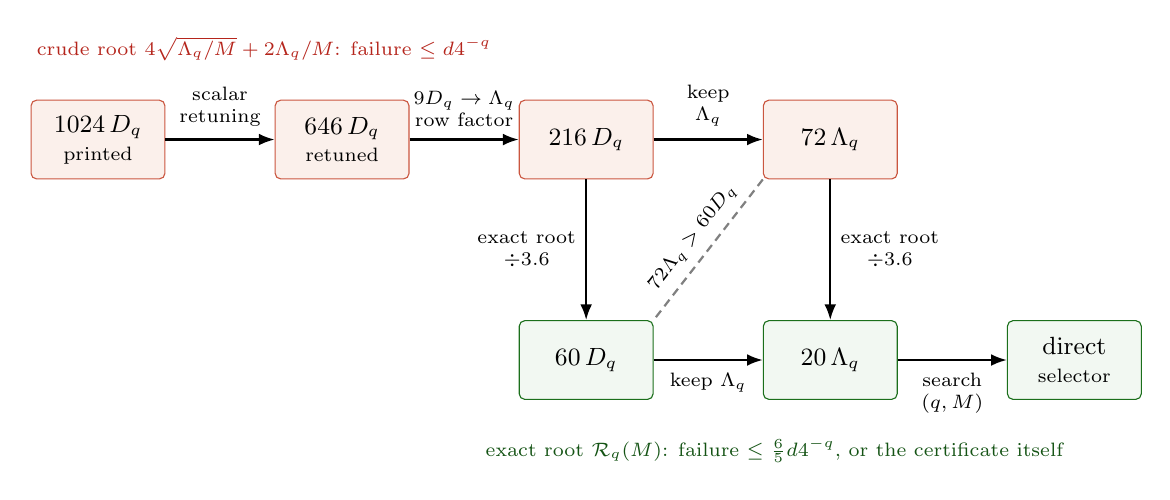
\begin{tikzpicture}[
  c/.style={draw,rounded corners=2pt,align=center,font=\small,minimum width=17mm,minimum height=10mm,inner sep=3pt},
  cr/.style={c,draw=BrickRed!70,fill=BrickRed!5},
  ex/.style={c,draw=ForestGreen!80!black,fill=ForestGreen!6},
  arr/.style={-{Latex[length=2mm]},thick},
  lab/.style={font=\scriptsize,align=center}]
\node[cr] (a) at (0,0) {$1024\,D_q$\\[-1pt]{\scriptsize printed}};
\node[cr] (b) at (3.1,0) {$646\,D_q$\\[-1pt]{\scriptsize retuned}};
\node[cr] (c) at (6.2,0) {$216\,D_q$};
\node[cr] (d) at (9.3,0) {$72\,\Lambda_q$};
\node[ex] (e) at (6.2,-2.8) {$60\,D_q$};
\node[ex] (f) at (9.3,-2.8) {$20\,\Lambda_q$};
\node[ex] (g) at (12.4,-2.8) {direct\\[-1pt]{\scriptsize selector}};
\draw[arr] (a)--node[lab,above=1pt]{scalar\\retuning}(b);
\draw[arr] (b)--node[lab,above=1pt]{$9D_q\to\Lambda_q$\\row factor}(c);
\draw[arr] (c)--node[lab,above=1pt]{keep\\$\Lambda_q$}(d);
\draw[arr] (c)--node[lab,left]{exact root\\$\div3.6$}(e);
\draw[arr] (d)--node[lab,right]{exact root\\$\div3.6$}(f);
\draw[arr] (e)--node[lab,below=1pt]{keep $\Lambda_q$}(f);
\draw[arr] (f)--node[lab,below=1pt]{search\\$(q,M)$}(g);
\draw[densely dashed,thick,Gray] (d.south west) -- node[lab,sloped,above,text=black]{$72\Lambda_q>60D_q$} (e.north east);
\node[lab,BrickRed,anchor=west] at (-0.9,1.15) {crude root $4\sqrt{\Lambda_q/M}+2\Lambda_q/M$: failure $\le d4^{-q}$};
\node[lab,ForestGreen!60!black,anchor=west] at (4.8,-3.95) {exact root $\Rex_q(M)$: failure $\le\tfrac65d4^{-q}$, or the certificate itself};
\end{tikzpicture}
\caption{The chain of sufficient row coefficients for the same two-round
fixed-size law. Top row: calibrations of the crude root. Bottom row:
calibrations of the exact root~\eqref{eq:exactroot}. Each vertical arrow
divides the coefficient by $3.6$; the dashed comparison is~\eqref{eq:chain}.}
\label{fig:chain}
\end{figure}

%======================================================================
\section{The direct deterministic selector}\label{sec:selector}

The certificate~\eqref{eq:cert} is an explicit function of $(q,M)$ and of the
known parameters. Nothing forces the root to be below $\eps/2$ or $q$ to equal
$q_*$; any pair with $\Cert(q,M)\le\delta$ is a valid prescription.
Algorithm~\ref{alg:selector} chooses the pair before any randomness is drawn.

\begin{algorithm}[t]
\caption{Direct selector for the two-round sketch}\label{alg:selector}
\begin{algorithmic}[1]
\Require $n,d,\eps,\delta,\alpha,\beta$; maximal order $q_{\max}$; safety margin $s\ge0$
\State $\mathrm{best}\gets(\bot,n)$ \Comment{$M=n$ is always exact}
\If{$q_{\max}\ge q_*$}
  \State $M_0\gets\min\{n,\lceil20\Lambda_{q_*}/\eps^2\rceil\}$
  \State $\mathrm{best}\gets(q_*,M_0)$ \Comment{proved canonical starting point}
\EndIf
\For{$q=1,\dots,q_{\max}$}
  \State compute $\Lambda_q$ from~\eqref{eq:allowances}
  \If{$\Cert(q,n-1)\le\delta$}
    \State $M_q\gets$ candidate in $[1,n-1]$ found by bisection \Comment{heuristic search}
    \State $M'\gets\min\{M_q+s,\,n-1\}$
    \If{$\Cert(q,M')\le\delta$ \textbf{and} $M'<\mathrm{best}.M$} \Comment{re-check at the final $M$}
       \State $\mathrm{best}\gets(q,M')$
    \EndIf
  \EndIf
\EndFor
\If{$\mathrm{best}.M=n$}
  \State \Return $M=n$, certificate $0$, no sign-independence requirement
\EndIf
\State \Return $\mathrm{best}=(q,M)$, $\Cert(q,M)$, and independence level $\min(n,4q)$
\end{algorithmic}
\end{algorithm}

The canonical starting point prevents the heuristic implementation from
returning a larger width than the canonical prescription when
$q_{\max}\ge q_*$. It does not certify that the returned width is globally
minimal. For a guaranteed minimum one must enumerate all candidate widths
or prove an appropriate monotonicity statement.

The atom $p_{n,M}$ should be evaluated through $\log\Gamma$ (or Stirling's
series) in high precision; the certificate is best handled as
$\log\Cert=\log d+2q\log(\Rex_q(M)/\eps)$.

\begin{proposition}[Validity and domination]\label{prop:selector}
\begin{enumerate}[label=(\roman*)]
\item If Algorithm~\ref{alg:selector} returns $(q,M)$ with $M<n$, then
$\Prob\{\norm{E_\cT}>\eps\}\le\Cert(q,M)\le\delta$ for every fixed isometry $U$,
under $\min(n,4q)$-wise independent signs. If it returns $M=n$ the embedding is
exact. Validity does not depend on the search being exact.
\item Let $M^\star=\min_{q\le q_{\max}}\min\{M<n:\Cert(q,M)\le\delta\}$ (or $n$
if this set is empty). If $q_{\max}\ge q_*$, then $M^\star$ is at most each of
$\lceil20\Lambda_{q_*}/\eps^2\rceil$ and $\lceil60D_{q_*}/\eps^2\rceil$, and at
most $\lceil72\Lambda_q/\eps^2\rceil$ and $\lceil216D_q/\eps^2\rceil$ for every
$q\le q_{\max}$ with $d4^{-q}\le\delta$, whenever these are below $n$.
\end{enumerate}
\end{proposition}
\begin{proof}
(i) is Theorem~\ref{thm:exactroot}, since the certificate is evaluated at the
returned $M$. (ii) For $M=\lceil20\Lambda_{q_*}/\eps^2\rceil<n$ the proof of
Theorem~\ref{thm:20} shows $\Rex_{q_*}(M)^{2q_*}\le\frac65(\eps/2)^{2q_*}$, so
$\Cert(q_*,M)\le\frac65d4^{-q_*}\le\delta$; the same holds for $60D_{q_*}$. For
$72\Lambda_q$ and $216D_q$, $\Rex_q\le\Rex_q^{\rm cr}\le\eps/2$ by the proof of
Corollary~\ref{cor:qf}, so $\Cert(q,M)\le d4^{-q}\le\delta$. Each is therefore a
feasible point of the minimization defining $M^\star$.
\end{proof}

\begin{remark}[Implementation]\label{rem:selector}
The stated root $\Rex_q(M)$ is not monotone in general. For example, take
$n=4$, $d=1$, $q=1$ and flat factors, so $\Lambda_1=25+2\sqrt{66}>36$.
Direct substitution gives
\[
 \Rex_1(2)=\frac85\sqrt{\Lambda_1},\qquad
 \Rex_1(3)=\frac{64}{37}\left(\sqrt{\Lambda_1/3}+\Lambda_1/6\right)
             >\Rex_1(2).
\]
Indeed $\Lambda_1/6>\sqrt{\Lambda_1}$ and $64/37>8/5$.
Both values in this example are outside the useful certification range;
it disproves global monotonicity without locating a nonmonotone feasible
interval. A returned $M$ must therefore not be rounded up (for
instance to a block size) without re-evaluating $\Cert$ at the new value, and
bisection is only a search heuristic; the final certificate check makes
every newly accepted candidate valid. The selected order may exceed $q_*$; under limited independence
the sign families must then be $\min(n,4q)$-wise independent ($72$-wise for
$q=18$). Fully independent signs are unaffected.
\end{remark}

At $n=2^{30}$, $\eps=1/2$, $\delta=0.01$ and flat transforms, with $s=10$, the
selector returns
\[
 (q,M)=(4,\,58\,406),\ (6,\,125\,760),\ (10,\,346\,325),\ (18,\,1\,423\,405)
 \quad\text{for } d=10,\,10^2,\,10^3,\,10^4,
\]
with certificates between $0.0099926$ and $0.0099986$. The least feasible
values are $58\,396$, $125\,750$, $346\,315$, $1\,423\,395$ (numerical; see
Section~\ref{sec:numerics}). At $d=10^4$ this is $35\%$ below
$20\Lambda_{q_*}$ and $48\%$ below $60D_{q_*}$.

%======================================================================
\section{Adaptive frames selected by randomly pivoted Cholesky}\label{sec:gate}

A fixed-subspace guarantee does not apply to a subspace chosen after looking at
the sketch. We allow one specific, useful form of dependence: a frame is
selected from a dictionary fixed in advance by running randomly pivoted
Cholesky (RP)~\cite{CETW} at full rank on a matrix that may depend on the
sketch arbitrarily, provided its range is fixed.

\paragraph{Setting.} Fix an isometry $V\in\C^{N\times k}$ and, for every
$k$-subset $J\subseteq[N]$ with $\det V_J\neq0$ ($V_J$ the rows of $V$ in $J$),
a target isometry $U_J\in\C^{n\times d}$, all before the sketch $S$ is drawn.
Let $C(S)\succ0$ be any measurable $k\times k$ matrix. Given $S$, run $k$ steps
of RP on $A_{\rm aux}=VC(S)V^*$ with fresh randomness: at a residual $R$, pick
the pivot $i$ with probability $R_{ii}/\tr R$ and replace $R$ by its Schur
complement. Release only the unordered pivot set $J$, and use the frame $U_J$.
The \emph{volume law} $\nu_V(J)=|\det V_J|^2$ is a probability distribution by
Cauchy--Binet and does not depend on $S$. For eigenvalues
$\lambda_1\ge\dots\ge\lambda_k>0$ of $C$ put
\begin{equation}\label{eq:gateprice}
 \tau_j(C)=\sum_{i>j}\lambda_i,\qquad
 \Gamma_C=\frac{k!\,\det C}{\prod_{j=0}^{k-1}\tau_j(C)} .
\end{equation}

\begin{proposition}[Likelihood price of the gate]\label{prop:gate}
Conditionally on $S$, the released law $\mu_{C(S)}$ satisfies
$\mu_{C(S)}(J)\le\Gamma_{C(S)}\,\nu_V(J)$ for every $J$, and $1\le\Gamma_C\le k!$.
If every fixed $U_J$ has sketch failure probability at most $\delta_0$ and
$\Gamma_{C(S)}\le\overline\Gamma$ almost surely, then the selected frame fails
with probability at most $\overline\Gamma\delta_0$.
\end{proposition}
\begin{proof}
\noindent\textbf{The pivot numerator is a determinant.}\enspace
An ordered pivot sequence $(j_1,\dots,j_k)$ with set $J$ has probability
\[
 \prod_{t=1}^k\frac{(R_{t-1})_{j_tj_t}}{\tr R_{t-1}}.
\]
Successive Schur complements give
\[
 \prod_{t=1}^k(R_{t-1})_{j_tj_t}
 =\det(A_{\rm aux})_{JJ}
 =\det C\,|\det V_J|^2.
\]

\noindent\textbf{Each denominator dominates a spectral tail.}\enspace
For the traces,
$A_{\rm aux}-R_t$ is the Nystr\"om approximation on $t$ columns, a PSD matrix
of rank at most $t$ dominated by $A_{\rm aux}$; with $P$ the projector onto its
range, $\tr(A_{\rm aux}-R_t)=\tr P(A_{\rm aux}-R_t)P\le\tr PA_{\rm aux}P\le
\lambda_1+\dots+\lambda_t$ by Ky Fan, since $A_{\rm aux}$ has eigenvalues
$\lambda_1,\dots,\lambda_k$ and zeros. Hence $\tr R_t\ge\tau_t(C)$, and every
ordered sequence has probability at most $\det C\,\nu_V(J)/\prod_t\tau_t(C)$.
Summing over the $k!$ orders gives $\mu_C(J)\le\Gamma_C\nu_V(J)$.
The range of the price follows because
$\lambda_{t+1}\le\tau_t(C)\le(k-t)\lambda_{t+1}$, multiplying over $t$ gives
$\det C\le\prod_t\tau_t\le k!\det C$, i.e.\ $1\le\Gamma_C\le k!$.

\noindent\textbf{Transfer the fixed-frame guarantee.}\enspace
Let $\mathsf B_J$ be the failure event of the fixed frame $U_J$, an event in
the sketch randomness. Then
\[
 \Prob\{\mathsf B_J\text{ for the selected }J\}
 =\E_S\sum_J\mu_{C(S)}(J)\mathbf 1_{\mathsf B_J}(S)
 \le\overline\Gamma\sum_J\nu_V(J)\Prob_S(\mathsf B_J)\le\overline\Gamma\delta_0,
\]
using that $\nu_V$ and the frames were fixed before $S$.
\end{proof}

The factorial comparison is Proposition~7 of Deshpande and
Vempala~\cite{DV}; $\Gamma_C$ retains its denominators. The same gate, with
the same price (written $\Lambda_C$ there), is used for sparse sketches
in~\cite{SparseCompanion}; we write $\Gamma_C$ to avoid a clash with the
allowance $\Lambda_q$. Nothing in Proposition~\ref{prop:gate} depends on the
sketch; only the fixed-frame guarantee it is combined with does. Flat $C$ gives
$\Gamma_C=1$ (full-rank RP on $VV^*$ is volume sampling~\cite{DRVW}). For a
spike $C=I+\eta uu^*$ ($\norm u=1$), $\Gamma_C=k(1+\eta)/(k+\eta)$. If the
eigenvalues are split into contiguous bands of sizes $n_\ell$ with
largest-to-smallest ratio at most $\varrho_\ell$ inside each band, bounding each
tail from below by the remaining eigenvalues of its own band gives
\begin{equation}\label{eq:bands}
 \Gamma_C\le\min\Bigl\{k!,\ \frac{k!}{\prod_\ell n_\ell!}\prod_\ell\varrho_\ell^{\,n_\ell}\Bigr\}.
\end{equation}

\begin{corollary}[SRHT on an RP-selected frame]\label{cor:gate}
In the setting above, let $0<\eps<1$, $0<\delta<1$, and let $\overline\Gamma$ be a
deterministic bound for $\Gamma_{C(S)}$ ($\overline\Gamma=k!$ is always allowed). Then
\[
 q=\Bigl\lceil\log_4\frac{6d\overline\Gamma}{5\delta}\Bigr\rceil,\qquad
 M=\min\{n,\lceil20\Lambda_q/\eps^2\rceil\}
\]
give $\Prob\{\norm{U_J^*S^*SU_J-I_d}>\eps\}\le\delta$ for the selected frame,
with $\min(n,4q)$-wise independent signs. Algorithm~\ref{alg:selector} run at
confidence $\delta/\overline\Gamma$ may be used instead.
\end{corollary}
\begin{proof}
Theorem~\ref{thm:20} with $\delta_0=\delta/\overline\Gamma$ and
Proposition~\ref{prop:gate}. When $M=n$ every frame is exact.
\end{proof}

Compared with the union bound over the dictionary, whose price can be
$\binom Nk$, the gate pays $\log\overline\Gamma\le\log k!$ inside $q$,
independently of $N$. For flat transforms this gives
$M=O(\eps^{-2}[d+(\log(d/\delta)+\log\overline\Gamma)^2])$.
Table~\ref{tab:gate} evaluates the example $d=100$, $k=10$, $N=1000$.

\begin{proposition}[Rank-two calibration]\label{prop:ranktwo}
For $k=2$, $\Gamma_C=2\lambda_1/(\lambda_1+\lambda_2)<2$ for every $C$, so
$\delta_0=\delta/2$ is always sufficient; with the canonical prescription this
is $q=\lceil\log_4(12d/(5\delta))\rceil$. A second-moment certificate
$\E_{\nu_V}(\mu_C/\nu_V)^2\le9/8$ would give, by Cauchy--Schwarz, failure at
most $\sqrt{9/8}\sqrt{\delta_0}$, i.e.\ the allowance $\delta_0=8\delta^2/9$.
The pointwise allowance is larger whenever $\delta<9/16$, so the
second-moment route is never useful in this range. For $k=1$ the gate equals
the volume law and costs nothing.
\end{proposition}
\begin{proof}
For $k=2$, $\Gamma_C=2\lambda_1\lambda_2/((\lambda_1+\lambda_2)\lambda_2)$.
The Cauchy--Schwarz bound is
$\E_{\nu}[(\mu/\nu)\mathbf 1_{\mathsf B}]\le(\E_\nu(\mu/\nu)^2)^{1/2}\Prob_\nu(\mathsf B)^{1/2}$.
Finally $\delta/2>8\delta^2/9$ iff $\delta<9/16$.
\end{proof}

\begin{remark}[Scope of the gate]
The range of $A_{\rm aux}$ must be fixed: if it could move with $S$, rank-one
inputs $e_{j(S)}e_{j(S)}^*$ would encode any label. The pivot order must not be
released, since it can carry extra information. The rank must be full, because
at partial rank the volume reference depends on $C$. The frame dictionary must
be fixed in advance. The bound $\overline\Gamma$ must hold uniformly; inserting
the observed $\Gamma_{C(S)}$ into a budget chosen after seeing the sketch is not
covered.
\end{remark}

%======================================================================
\section{Whole-sketch Nystr\"om energy}\label{sec:nystrom}

Throughout this section $K\in\C^{n\times n}$ is Hermitian positive
semidefinite, $G=S^*S$ and
\[
 \Nys_K(S^*)=KS^*(SKS^*)^\dagger SK,\qquad R=K-\Nys_K(S^*).
\]
Rescaling $S$ by a scalar does not change $\Nys_K(S^*)$, but it changes $G$;
we use the normalization~\eqref{eq:sketch}, for which $\E G=I$. Put
$z_j=\sqrt n\,Q^*e_j$, so that $G=M^{-1}\sum_{j\in\cT}z_jz_j^*$ and
$\sum_{j=1}^nz_jz_j^*=nI$.

\begin{lemma}[Deterministic Gram-error comparison]\label{lem:det}
For every sketch $S$,
\[
 0\preceq R\preceq K,\qquad R\preceq(I-G)K(I-G),\qquad
 \norm R_F^2\le\tr(KR)\le\tr[K(I-G)K(I-G)] .
\]
\end{lemma}
\begin{proof}
\noindent\textbf{Represent the residual by a projector.}\enspace
Let $P$ be the orthogonal projector onto $\range(K^{1/2}S^*)$.
The identity $X(X^*X)^\dagger X^*=P_{\range X}$ gives
\[
 \Nys_K(S^*)=K^{1/2}PK^{1/2},\qquad
 R=K^{1/2}(I-P)K^{1/2}.
\]
Thus $0\preceq R\preceq K$.

\noindent\textbf{Insert the Gram error.}\enspace
Since $(I-P)K^{1/2}S^*=0$, we have $RG=GR=0$. Consequently
\[
 R=(I-G)R(I-G)\preceq(I-G)K(I-G).
\]
The inequalities for the traces now follow from positivity:
\[
 \tr(R^2)\le\tr(KR)
 \le\tr\!\left[K^{1/2}(I-G)K(I-G)K^{1/2}\right].
\]
The first step uses $\tr[R(K-R)]\ge0$; the second uses the preceding
Loewner comparison after congruence by $K^{1/2}$.
\end{proof}

\begin{lemma}[Finite-population identity]\label{lem:population}
Let $n\ge2$, $1\le M\le n$, and fix the unitary $Q$. For every Hermitian $X$,
\[
 \E_\cT[(G-I)X(G-I)]=\lambda_{n,M}\Bigl(\frac1n\sum_{j=1}^nz_jz_j^*Xz_jz_j^*-X\Bigr).
\]
In particular
$\E_\cT\tr[K(G-I)K(G-I)]=\lambda_{n,M}\bigl[n^{-1}\sum_j(z_j^*Kz_j)^2-\norm K_F^2\bigr]$.
\end{lemma}
\begin{proof}

For a uniform $M$-subset,
\[
 \Prob(j\in\cT)=\frac Mn,\qquad
 \Prob(j,l\in\cT)=\frac{M(M-1)}{n(n-1)}\quad(j\ne l).
\]
Define $W=\sum_jz_jz_j^*Xz_jz_j^*$. Since
$\sum_jz_jz_j^*=nI$, the off-diagonal part of the double sum is
\[
 \sum_{j\ne l}z_jz_j^*Xz_lz_l^*=n^2X-W.
\]
The two inclusion probabilities now give
\begin{align*}
 \E_\cT GXG
 &=\frac{W}{Mn}+\frac{M-1}{Mn(n-1)}(n^2X-W)\\
 &=\frac{\lambda_{n,M}}nW+(1-\lambda_{n,M})X.
\end{align*}
Because $\E_\cT G=I$, expanding $(G-I)X(G-I)$ subtracts $X$ from this
expression. Taking $\tr(K\,\cdot)$ with $X=K$ proves the scalar identity.

\end{proof}

\begin{lemma}[Rademacher fourth moments]\label{lem:rad4}
Let $\epsilon\in\{\pm1\}^n$ be four-wise independent and unbiased. For
Hermitian $C$,
$\E(\epsilon^{\mathsf T}C\epsilon)^2=(\tr C)^2+2\norm{\Re C}_F^2-2\sum_aC_{aa}^2
\le(\tr C)^2+2\norm C_F^2$. For real symmetric $C$,
$\E[\epsilon\epsilon^{\mathsf T}C\epsilon\epsilon^{\mathsf T}]=(\tr C)I+2C-2\Diag(C)$.
\end{lemma}
\begin{proof}
$\E\epsilon_a\epsilon_b\epsilon_c\epsilon_d=\delta_{ab}\delta_{cd}+\delta_{ac}\delta_{bd}
+\delta_{ad}\delta_{bc}-2\mathbf 1_{a=b=c=d}$. Hence
$\E(\epsilon^{\mathsf T}C\epsilon)^2=(\tr C)^2+\sum_{ab}(C_{ab}^2+|C_{ab}|^2)-2\sum_aC_{aa}^2$,
and $\sum_{ab}(C_{ab}^2+|C_{ab}|^2)=2\norm{\Re C}_F^2$ because $C_{ba}=\overline{C_{ab}}$.
The matrix identity is the same expansion with free indices.
\end{proof}

\begin{theorem}[One actual two-round sketch]\label{thm:whole}
Let $A$ be flat and $B$ unitary, let $D_x,D_y$ be four-wise independent,
mutually independent and independent of $\cT$, and let $n\ge2$.
\begin{enumerate}[label=(\alph*)]
\item $\E\norm{K-\Nys_K(S^*)}_F^2\le\E\tr[K(G-I)K(G-I)]\le
\lambda_{n,M}\bigl[(\tr K)^2+\norm K_F^2\bigr]$.
\item If $K$ is real and $A,B$ are real flat orthogonal matrices, then
\begin{equation}\label{eq:twoexact}
 \E\tr[K(G-I)K(G-I)]=\lambda_{n,M}\Bigl[\Bigl(1-\frac2n\Bigr)(\tr K)^2
 +\Bigl(1-\frac4n\Bigr)\norm K_F^2+\frac4n\sum_iK_{ii}^2\Bigr],
\end{equation}
and consequently
\begin{equation}\label{eq:simple}
 \E\norm{K-\Nys_K(S^*)}_F^2\le\frac2M\Bigl(1-\frac Mn\Bigr)(\tr K)^2 .
\end{equation}
\end{enumerate}
No independence between the sampled rows is assumed; they share both sign
diagonals.
\end{theorem}
\begin{proof}

\noindent\textbf{General unitary inner transform.}\enspace
The deterministic comparison is Lemma~\ref{lem:det}. To compute the
remaining energy, fix a row $j$ and condition on $D_x$. Define
\[
 V=BD_x,\qquad h=\sqrt n\,A^*e_j,\qquad
 C=D_h^*VKV^*D_h.
\]
Flatness of $A$ makes every entry of $h$ unimodular. Therefore
$z_j=V^*D_hy$, and $C$ is unitarily similar to $K$. In particular,
\[
 z_j^*Kz_j=y^{\mathsf T}Cy,
 \qquad \tr C=\tr K,\qquad \norm C_F=\norm K_F.
\]
The Rademacher identity of Lemma~\ref{lem:rad4} gives
\[
 \E(z_j^*Kz_j)^2\le(\tr K)^2+2\norm K_F^2.
\]
Averaging this inequality over the rows and using
Lemma~\ref{lem:population} proves part (a). The population identity
subtracts one copy of $\norm K_F^2$, which explains the final coefficient
of that term.

\noindent\textbf{Exact energy for real flat transforms.}\enspace
Assume now that $A,B,K$ are real and both transforms are flat.
The entries of $h$ are signs, so multiplying $y$ by $D_h$ preserves
its four-wise independent Rademacher law. Conditional expectation over $y$
thus gives the equality
\[
 \E_y(z_j^{\mathsf T}Kz_j)^2
 =(\tr K)^2+2\norm K_F^2
     -2\sum_a(VKV^{\mathsf T})_{aa}^2.
\]
It remains to average the last sum over the inner signs $x$.
For each $a$, write
\[
 (VKV^{\mathsf T})_{aa}=x^{\mathsf T}C^{(a)}x,
 \qquad C^{(a)}_{il}=B_{ai}K_{il}B_{al}.
\]
Since $B_{ai}^2=1/n$, the three quantities in the fourth-moment formula are
\[
 \tr C^{(a)}=\frac{\tr K}{n},\qquad
 \norm{C^{(a)}}_F^2=\frac{\norm K_F^2}{n^2},\qquad
 \sum_i(C^{(a)}_{ii})^2=\frac{\sum_iK_{ii}^2}{n^2}.
\]
Applying Lemma~\ref{lem:rad4} a second time and summing over $a$ yields
\[
 \E_x\sum_a(VKV^{\mathsf T})_{aa}^2
 =\frac1n\left[(\tr K)^2+2\norm K_F^2-2\sum_iK_{ii}^2\right].
\]
This value is independent of $j$. Substitute it into the preceding
conditional identity, then apply Lemma~\ref{lem:population}; the result
is~\eqref{eq:twoexact}.

\noindent\textbf{A bound depending only on the trace.}\enspace
Set $T=\tr K$, $F=\norm K_F^2$, and $\Delta=\sum_iK_{ii}^2$.
Positivity gives $\Delta\le F\le T^2$. For $n\ge4$,
\[
 (1-4/n)F+(4/n)\Delta\le F\le T^2.
\]
For $n<4$, the coefficient of $F$ is negative; using $F\ge\Delta$
instead gives the same upper bound. Thus the bracket in
\eqref{eq:twoexact} is at most $(2-2/n)T^2$. Finally,
\[
 \lambda_{n,M}(2-2/n)=\frac2M(1-M/n),
\]
which proves~\eqref{eq:simple}.

\end{proof}

\begin{theorem}[The one-round law]\label{thm:oneround}
For the one-round sketch $S=\sqrt{n/M}\,R_\cT AD_x$ with $A$ real flat
orthogonal, $D_x$ four-wise independent and $K$ real,
\[
 \E\tr[K(G-I)K(G-I)]=\lambda_{n,M}\Bigl[(\tr K)^2+\norm K_F^2-2\sum_iK_{ii}^2\Bigr],
\]
and~\eqref{eq:simple} holds. Part (a) of Theorem~\ref{thm:whole} also covers
this law (take $B=I$).
\end{theorem}
\begin{proof}
Here $z_j=D_xh$ with $h\in\{\pm1\}^n$, and Lemma~\ref{lem:rad4} with
$C=D_hKD_h$ gives $\E(z_j^{\mathsf T}Kz_j)^2=T^2+2F-2\Delta$; apply
Lemma~\ref{lem:population}. Since $F\le T^2$ and $\Delta\ge T^2/n$ by
Cauchy--Schwarz, $T^2+F-2\Delta\le(2-\frac2n)T^2$.
\end{proof}

\begin{remark}[Neither law dominates; rank blindness]\label{rem:blind}
The one-round bracket minus the two-round bracket is
$\frac2n(T^2+2F)-2(1+\frac2n)\Delta$, which has either sign. For $K=e_1e_1^{\mathsf T}$
the one-round energy vanishes while the two-round energy is
$\lambda_{n,M}(2-\frac2n)$; for $K=\mathbf 1\mathbf 1^{\mathsf T}/n$ the two-round
energy $\lambda_{n,M}(2-\frac6n+\frac4{n^2})$ is the smaller one. Both satisfy the same
final bound~\eqref{eq:simple}.

The quantity $\tr[K(G-I)K(G-I)]=\norm{K^{1/2}S^*SK^{1/2}-K}_F^2$ is the
approximate-matrix-multiplication error for the product $K^{1/2}\cdot K^{1/2}$
under without-replacement row sampling, and~\eqref{eq:simple} is the
corresponding variance scale $\norm{K^{1/2}}_F^4/M=(\tr K)^2/M$ of Drineas,
Kannan and Mahoney~\cite{DKM}. Our bound has coefficient $2$ and the
finite-population factor $1-M/n$. It
does not see the rank or the spectral decay of $K$: in the enumeration of
Section~\ref{sec:numerics} a rank-three $K$ at $n=8$, $M=3$ has expected
Nystr\"om residual $20.0$ against the bound $4250$. The theorem is therefore an
$O((\tr K)^2/M)$ statement of approximate-matrix-multiplication type, not a relative-error
Nystr\"om guarantee; its value is that it applies to one sketch with shared
signs and is exact at $M=n$.

There is also a structural reason to distinguish expected and
high-probability tail-relative guarantees. The finite-support obstruction
in~\cite[proposition on expected tail-relative guarantees]{SparseCompanion}
applies to the present real flat law whenever $M<n$.
Choose a sketch value $S_0$ of positive probability and a unit vector
$u\in\ker S_0$. For $K_H=Huu^{\mathsf T}+I_n$, the spectral tail after
rank $r\ge1$ is $n-r$, independent of $H$, but on the event $S=S_0$ the
Nystr\"om residual retains eigenvalue $H+1$ along $u$. Its expected trace
and squared Frobenius norm therefore grow without bound as $H\to\infty$.
A uniform expected bound depending only on that tail is impossible.
High-probability statements can instead allocate this event to their
failure budget.
\end{remark}

\subsection{Trace and diagonal estimation}

\begin{corollary}[Sketch-and-correct trace estimator]\label{cor:trace}
Let $\widehat K=\Nys_K(S^*)$ be built from $M$ matrix--vector products with an
$M$-row sketch satisfying~\eqref{eq:simple}, and let $\xi_1,\dots,\xi_t$ be
independent Rademacher vectors, independent of $S$. The estimator
\[
 \widehat T=\tr\widehat K+\frac1t\sum_{\ell=1}^t\xi_\ell^{\mathsf T}(K-\widehat K)\xi_\ell
\]
uses $M+t$ matrix--vector products, all chosen before any response is seen, and
satisfies
\[
 \E\widehat T=\tr K,\qquad \Var\widehat T\le\frac2t\E\norm{K-\widehat K}_F^2
 \le\frac{4(1-M/n)}{Mt}(\tr K)^2 .
\]
With $M=\min\{n,\lceil2\sqrt3/\eps\rceil\}$ and
$t=\lceil2\sqrt3/\eps\rceil$ (the case $M=n$ is exact), $|\widehat T-\tr K|\le\eps\tr K$
with probability at least $2/3$.
\end{corollary}
\begin{proof}
Conditionally on $S$, $\widehat T$ is unbiased for $\tr K$ and has variance
$t^{-1}(2\norm{K-\widehat K}_F^2-2\sum_i(K-\widehat K)_{ii}^2)$ by
Lemma~\ref{lem:rad4}. The law of total variance and~\eqref{eq:simple} give the
bound, and Chebyshev's inequality with $Mt\ge12/\eps^2$ gives the last claim.
The quantities $\tr\widehat K$ and $\xi^{\mathsf T}\widehat K\xi$ are computed
from $KS^*$ alone.
\end{proof}
The $O(1/\eps)$ query count is that of Hutch++~\cite{Hutchpp}; the point here
is that the two-round transform realizes it with one fixed-size sketch.
The Nystr\"om approximation plus residual correction is the construction
of Nystr\"om++~\cite{Nystrompp}, rather than a new estimator architecture.

\begin{proposition}[Covariance map]\label{prop:covmap}
Let $X$ be real symmetric and $1\le m\le n$, and let $G_0=S_0^{\mathsf T}S_0$ for
an $m$-row sketch. For the real flat two-round law,
\[
 \E[(G_0-I)X(G_0-I)]=\lambda_{n,m}\Bigl[\Bigl(1-\frac4n\Bigr)X
 +\Bigl(1-\frac2n\Bigr)(\tr X)I+\frac4n\Diag(X)\Bigr],
\]
and for the real flat one-round law
$\E[(G_0-I)X(G_0-I)]=\lambda_{n,m}[X+(\tr X)I-2\Diag(X)]$.
\end{proposition}
\begin{proof}

By Lemma~\ref{lem:population}, it suffices to compute the one-row map
$\E[z_jz_j^{\mathsf T}Xz_jz_j^{\mathsf T}]$. The finite-population correction
then subtracts $X$ and multiplies by $\lambda_{n,m}$.

For the two-round law, condition on $x$ and set $V=BD_x$.
Then $z_j=V^{\mathsf T}\epsilon$ for a four-wise independent sign vector
$\epsilon$. The matrix fourth-moment identity gives
\[
 \E_y[z_jz_j^{\mathsf T}Xz_jz_j^{\mathsf T}]
 = (\tr X)I+2X-2V^{\mathsf T}\Diag(VXV^{\mathsf T})V.
\]
The $(i,l)$ entry of the last term before its factor $-2$ is
\[
 x_ix_l\sum_aB_{ai}B_{al}
               \sum_{u,v}B_{au}x_uX_{uv}x_vB_{av}.
\]
Apply the four-point sign formula to $x_ix_lx_ux_v$, using
$B_{ai}^2=1/n$. This gives
\[
 \E_x[V^{\mathsf T}\Diag(VXV^{\mathsf T})V]_{il}
 =\frac1n\left[(\tr X)\delta_{il}+2X_{il}-2\delta_{il}X_{ii}\right].
\]
Consequently the unconditional one-row map is
\[
 (1-2/n)[(\tr X)I+2X]+(4/n)\Diag(X).
\]
Subtracting $X$ proves the two-round formula.

For the one-round law, $z_j=D_hx$ with $h$ a fixed sign vector.
The fourth-moment identity directly gives the one-row map
$(\tr X)I+2X-2\Diag(X)$. Again subtract $X$ and apply the
finite-population factor.

\end{proof}

\begin{corollary}[Sketch-and-correct diagonal estimator]\label{cor:diag}
Let $K$ be real, $\widehat K$ as in Corollary~\ref{cor:trace}, and let $S_0$ be an
independent $m$-row sketch of either real flat law. Then
$\widehat d=\diag(\widehat K)+\diag\bigl((K-\widehat K)S_0^{\mathsf T}S_0\bigr)$ uses
$M+m$ matrix--vector products, is unbiased for $\diag K$, and
\[
 \E\norm{\widehat d-\diag K}_2^2\le\frac2m\Bigl(1-\frac mn\Bigr)
 \E\norm{K-\widehat K}_F^2
 \le\frac4{mM}\Bigl(1-\frac mn\Bigr)\Bigl(1-\frac Mn\Bigr)(\tr K)^2 .
\]
\end{corollary}
\begin{proof}
Condition on $\widehat K$ and put $X=K-\widehat K$, $r_i=Xe_i$. The error in
coordinate $i$ is $r_i^{\mathsf T}(G_0-I)e_i$, whose second moment is
$e_i^{\mathsf T}\E[(G_0-I)r_ir_i^{\mathsf T}(G_0-I)]e_i$. By
Proposition~\ref{prop:covmap} this equals
$\lambda_{n,m}[X_{ii}^2+(1-\frac2n)\norm{r_i}^2]$ for the two-round law and
$\lambda_{n,m}[\norm{r_i}^2-X_{ii}^2]$ for the one-round law. Summing over $i$,
the total is at most $\lambda_{n,m}(2-\frac2n)\norm X_F^2=\frac2m(1-\frac mn)\norm X_F^2$.
Now apply~\eqref{eq:simple}.
\end{proof}
With $M=m=\min\{n,\lceil2\sqrt3/\eps\rceil\}$, using exact recovery if this equals $n$,
the bound gives $\norm{\widehat d-\diag K}_2\le\eps\tr K$
with probability at least $2/3$, the guarantee of Diag++~\cite{BN}. The
two-round law has a nonzero error even for diagonal $X$ (the term $X_{ii}^2$),
which the one-round law does not.

%======================================================================
\section{Fresh-row drift}\label{sec:drift}

\begin{lemma}[One Khintchine factor]\label{lem:row}
Let $A$ be flat, $B$ unitary, the signs fully independent, $j$ fixed and
$z=\sqrt n\,Q^*e_j$. Then $\E zz^*=I$, and for $p\ge1$, $u\in\C^n$, $X\succeq0$,
\[
 \E|u^*z|^{2p}\le g(p)\norm u^{2p},\qquad \E(z^*Xz)^p\le g(p)(\tr X)^p,\qquad
 g(p)=\frac{2^p\Gamma(p+\frac12)}{\sqrt\pi}.
\]
\end{lemma}
\begin{proof}
Condition on $D_x$ and put $v=BD_xu$. Then
$\overline{u^*z}=\sqrt n\,(Qu)_j=\sum_a y_a\,c_a$ with $c_a=\sqrt n\,A_{ja}v_a$,
and $\sum_a|c_a|^2=\norm v^2=\norm u^2$ by flatness. The
same computation gives $\E_yzz^*=I$. \noindent\textbf{Linear moment bound.}\enspace
For real coefficients, the sharp
Khintchine inequality of Haagerup~\cite{Haagerup} (for exponents in $(2,3)$ see
also Mordhorst~\cite{Mordhorst}) gives
$\E|\sum_ay_ac_a|^{2p}\le\E|g|^{2p}\norm c^{2p}$ with $g$ standard Gaussian, and
$\E|g|^{2p}=g(p)$. For complex coefficients apply it to the real and imaginary
parts and Minkowski's inequality in $L^p$ to
$|\sum y_ac_a|^2=(\sum y_a\Re c_a)^2+(\sum y_a\Im c_a)^2$. \noindent\textbf{Quadratic moment bound.}\enspace
Write $X=\sum_i\mu_iu_iu_i^*$ with orthonormal $u_i$ and $\mu_i\ge0$.
Minkowski's inequality and the linear bound give
\[
 \|(z^*Xz)\|_{L^p}
 \le\sum_i\mu_i\,\||u_i^*z|^2\|_{L^p}
 \le g(p)^{1/p}\sum_i\mu_i.
\]
Taking the $p$th power gives the stated bound.
\end{proof}

Since $g(1)=1$ and $\frac{d}{dp}\log g(p)|_{p=1}=\log2+\psi(3/2)=2-\gamma-\log2$,
\begin{equation}\label{eq:kappa0}
 \kappa_0:=\lim_{\beta\downarrow0}g(1+\beta)^{1/\beta}=\frac{e^{2-\gamma}}2
 =2.0743278106\ldots,
\end{equation}
where $\gamma$ is Euler's constant.

\begin{lemma}[Ratio conversion; the argument of~\cite{PP}]\label{lem:ratio}
Let $z$ be isotropic with $\E|u^*z|^{2p}\le H(p)\norm u^{2p}$ and
$\E(z^*Xz)^p\le H(p)(\tr X)^p$ at $p=1+\beta$, $\beta>0$. For nonzero PSD
$Y,R$ with $\ker R\subseteq\ker Y$,
\[
 \E\frac{z^*Yz}{z^*Rz}\ge\frac{\tr Y}{H(1+\beta)^{1/\beta}\tr R}
\]
(the quotient being $0$ when $z^*Rz=0$).
\end{lemma}
\begin{proof}

Set $a=z^*Yz$ and $b=z^*Rz$. The kernel condition ensures $a=0$ whenever
$b=0$, while isotropy gives $\E a=\tr Y$. Introduce the probability measure
\[
 dQ=\frac{a}{\tr Y}\,d\Prob.
\]
Under $Q$, the variable $b$ is positive almost surely. Jensen's inequality
for $t\mapsto t^{-1/\beta}$ therefore gives
\[
 \E\frac ab=\tr Y\,\E_Qb^{-1}
 \ge\tr Y\,(\E_Qb^\beta)^{-1/\beta}.
\]
It remains to bound the last expectation. Write
$Y=\sum_i\mu_iu_iu_i^*$ with orthonormal $u_i$ and $\mu_i\ge0$.
H\"older's inequality with exponents $p=1+\beta$ and $p/\beta$ gives
\begin{align*}
 \E[|u_i^*z|^2b^\beta]
 &\le(\E|u_i^*z|^{2p})^{1/p}(\E b^p)^{\beta/p}\\
 &\le H(p)(\tr R)^\beta.
\end{align*}
Multiply by $\mu_i$, sum over $i$, and divide by $\tr Y$ to obtain
$\E_Qb^\beta\le H(p)(\tr R)^\beta$. Substitution proves the claim.

\end{proof}

\begin{theorem}[Fresh-row drift]\label{thm:drift}
Let $z$ be as in Lemma~\ref{lem:row}, $R_0\succeq0$ nonzero and
$R_1=R_0-R_0z(z^*R_0z)^\dagger z^*R_0$. Then $0\preceq R_1\preceq R_0$ and
\[
 \E(\tr R_0-\tr R_1)\ge\frac{\tr(R_0^2)}{\kappa_0\tr R_0}.
\]
If $R_k$ is obtained from $K\succeq0$ by $k$ such updates with independent fresh
draws of $(D_x,D_y)$, then $\E\norm{R_k}_F^2\le\kappa_0(\tr K)^2/k$.
\end{theorem}
\begin{proof}
The trace drop is $z^*R_0^2z/z^*R_0z$. Apply Lemma~\ref{lem:ratio} with
$Y=R_0^2$, $R=R_0$, $H=g$, and let $\beta\downarrow0$ using~\eqref{eq:kappa0}.
For the second claim, conditioning gives
$\E[\tr R_t-\tr R_{t+1}\mid R_t]\ge\tr(R_t^2)/(\kappa_0\tr K)$; summing,
$\sum_{t<k}\E\tr(R_t^2)\le\kappa_0(\tr K)^2$, and $\tr(R_t^2)$ is nonincreasing
because $R_{t+1}\preceq R_t$.
\end{proof}

\begin{remark}[What the constant means]
The constant $\kappa_0$ is exactly the constant of an i.i.d.\ Rademacher probe,
which satisfies the same Khintchine envelope, costs $O(n)$ and needs no
flatness. Theorem~\ref{thm:drift} therefore says that a fresh row of the
two-round transform is no worse than a Rademacher probe, and in particular that
the two transforms do not square the constant. It is not an algorithmic gain
over Rademacher probing; the SRHT-specific content is in
Theorem~\ref{thm:whole}. The theorem does not justify charging the $M$ rows of
one sketch as $M$ independent updates, since they share $D_x,D_y$. Finite
spherical constants do not transfer either: at $n=2$, $H_2D_yH_2$ is a signed
identity or a signed swap, so $|e_1^*z|^2\in\{0,2\}$ equiprobably and the
order-one constant of this law is $2$, above the value $e/2$ of the
two-dimensional real sphere. For a nonflat outer transform and a uniformly random
row $J$, the same proof with $H(p)=g(p)\alpha^{p-1}$ gives the constant
$\alpha\kappa_0$.
\end{remark}

%======================================================================
\section{Sketched randomly pivoted Cholesky}\label{sec:sketchedrp}

Let $F\in\R^{D\times N}$ and $A=F^{\mathsf T}F$. \emph{Sketched RP} runs RP on
$B=(\Pi F)^{\mathsf T}(\Pi F)$ for a random sketch $\Pi$ with $D$ columns and
measures the error on $A$. In \emph{RPCholesky under approximate and sketched
pivot probabilities}~\cite{RobustRP} it is shown that one does not need an
embedding of $\range F$: it suffices that $\Pi$ embeds, with a failure
probability small against the RP path likelihood, the spans of the pivot columns
actually reached, augmented by one direction. This section records what the
two-round transform supplies to that framework.

\begin{definition}[Path-local moment property]
A random $\Pi\in\C^{M\times D}$ has the moment property $(\ell,q,\eps_0,C_0)$ if
$\E\tr(U^*\Pi^*\Pi U-I_d)^{2q}\le C_0\,d\,\eps_0^{2q}$ for every fixed isometry
$U\in\C^{D\times d}$ with $d\le\ell$.
\end{definition}

\begin{proposition}[The two-round transform]\label{prop:pathlocal}
Let $0<\eps_0<1/2$, $\ell\ge1$, $q\ge1$, and let $\Lambda_q(\ell)$ denote
$\Lambda_q$ with $d=\ell$. The two-round sketch on $\C^D$ with
$M\ge\min\{D,\lceil5\Lambda_q(\ell)/\eps_0^2\rceil\}$ rows has the moment property
$(\ell,q,\eps_0,6/5)$, under $\min(D,4q)$-wise independent signs.
\end{proposition}
\begin{proof}
$\Lambda_q$ is increasing in $d$, and $5\Lambda_q(\ell)/\eps_0^2=20\Lambda_q(\ell)/(2\eps_0)^2$.
Apply~\eqref{eq:20moment} with $\eps=2\eps_0<1$ to each $d\le\ell$.
\end{proof}

\begin{imported}[Sketched RP, conservative path interface;~\cite{RobustRP}]\label{imp:sketchedrp}
Let $1\le r<k$, $\tau=\tau_r(A)>0$, $0<\eps\le1$ and $0<\eta\le1/4$, and write
$R_A(J)=A-A_{:,J}A_{JJ}^\dagger A_{J,:}$. If $\Pi$ is independent of the
pivoting randomness and has the moment property $(k+1,q,\eps_0,C_0)$ with
$q\ge\max\{2,k\}$ and $\eps_0\le\eta/2$, then on a good event for the current pivot set $J$ the
sketched residual trace satisfies
$(1-\eta-\eta^2)\tr R_A(J)\le\tr R_B(J)\le(1+\eta)\tr R_A(J)$, and the expected
decrease of $\tr R_A$ in one sketched step is at least
$\gamma\,\tr(R_A^2)/\tr R_A$ with $\gamma=(1-\eta-\eta^2)/(1+\eta)$. Hence
the recurrence argument for randomly pivoted Cholesky~\cite{CETW}, run
with the factor $\gamma$ as in~\cite{RobustRP}, gives
$\E\tr R_A(J_k)\le(1+\eps)\tau+\tr(A)\,P_{\rm fail}$, for instance for
$k\ge\lceil(r/\gamma)(\eps^{-1}+\log\eps^{-1}+\log(\tr A/\tau))\rceil$.
The path second-moment estimate gives the explicit failure bound
\[
 P_{\rm fail}\le
 \min\!\left\{1,\,2(k+1)e^{k\chi_\eta^2/2}C_0^{1/2}2^{-q/2}\right\},
 \qquad \chi_\eta=\frac{2\eta}{1-\eta}.
\]
The hypotheses and the exhausted-residual convention are given
in~\cite{RobustRP}. The same sketch can be reused for the
reconstruction $F\approx F_J(\Pi F_J)^\dagger\Pi F$.
\end{imported}

\begin{remark}[Rows scale quadratically in the pivot budget]
For $\eps_0=\eta/2$ and $C_0=6/5$, the explicit path bound makes
$\tr(A)P_{\rm fail}\le\eps\tau$ whenever
\[
 q\ge\max\!\left\{2,k,\,
 \frac{k\chi_\eta^2}{\log2}
 +2\log_2\!\frac{2(k+1)\sqrt{6/5}\,\tr A}{\eps\tau}\right\}.
\]
The constraint $q\ge k$ covers the determinant path estimate;
it remains in this conservative interface even when the likelihood exponent is small.
Thus a sufficient order is $O(k+\log(k\tr A/(\eps\tau)))$.
For the two-round transform with flat factors,
$\Lambda_q(k+1)\ge2(k+1)+22q^2-q$, so Proposition~\ref{prop:pathlocal} gives
$M=O(\eta^{-2}[k+(k+\log(k\tr A/(\eps\tau)))^2])$ rows: quadratic in $k$ at
fixed $\eta$, whereas a sketch with allowance linear in $q$ gives rows linear in
$k$. The uncapped sufficient budget is independent of $N$ and $D$.
The hybrid path comparison in~\cite{RobustRP} can instead use $q\ge2$
and order $O(\eta^2k+\log(k\tr A/(\eps\tau)))$; its SRHT budget is still
quadratic in $k$ at fixed $\eta$. Numerically, at $\eta=1/4$
($\eps_0=1/8$) and $q=\ell$, Proposition~\ref{prop:pathlocal} asks for
$M/\ell^2\approx1.1\times10^4$ for $\ell=11,51,101$
(Section~\ref{sec:numerics}); this is a scope theorem, useful only for very tall $F$.
\end{remark}


%======================================================================
\section{Numerical evaluation}\label{sec:numerics}

The original tables were computed in Julia with $256$-bit
floating point; the scripts are supplied in \texttt{checks/original/}.
An independent Python audit in \texttt{checks/audit\_srht.py} recomputes
the scalar prescriptions, certificate boundaries, and representative
whole-sketch identities. These are numerical checks of the stated formulas,
not a formal verification of the imported operator results.

In the original computation, binomial atoms were evaluated from exact log-factorials
(Stirling's series with remainder below $10^{-30}$ for arguments above
$10^3$). They evaluate the sufficient conditions proved above and are not
empirical thresholds. Unless stated otherwise the transforms are flat,
$n=2^{30}$ (no prescription is capped), $\eps=1/2$ and $\delta=0.01$; then
$q=\lceil\log_4(400d)\rceil$ is the order of~\cite{V11,HY},
$q_*=\lceil\log_4(120d)\rceil$ and $q_f=\lceil\log_4(100d)\rceil$.

\begin{table}[ht]
\centering\small
\setlength{\tabcolsep}{4.5pt}
\begin{tabular}{rrrrrrrrr}
\toprule
$d$ & $q/q_*$ & $216D_q$ & $72\Lambda_q$ & $60D_{q_*}$ & $20\Lambda_{q_*}$ &
direct $M$ & $q$ (indep.) & least feasible\\
\midrule
10 & 6/6 & 381\,888 & 369\,386 & 106\,080 & 102\,608 & 58\,406 & 4 (16) & 58\,396\\
100 & 8/7 & 749\,952 & 717\,818 & 165\,120 & 157\,664 & 125\,760 & 6 (24) & 125\,750\\
1\,000 & 10/9 & 1\,900\,800 & 1\,733\,312 & 473\,280 & 427\,412 & 346\,325 & 10 (40) & 346\,315\\
10\,000 & 11/11 & 9\,894\,528 & 7\,894\,646 & 2\,748\,480 & 2\,192\,958 & 1\,423\,405 & 18 (72) & 1\,423\,395\\
\bottomrule
\end{tabular}
\caption{Sufficient row counts. The first two columns after $q/q_*$ calibrate the
crude root at the order $q$ of~\cite{V11,HY}; the next two the exact root at
$q_*$. ``Direct'' is the output of Algorithm~\ref{alg:selector} with safety
margin $s=10$, its order and the required sign independence $\min(n,4q)$; the
certificates at the returned $M$ are $0.0099926$, $0.0099947$, $0.0099969$,
$0.0099986$. ``Least feasible'' is the smallest $M$ with $\Cert(q,M)\le\delta$
for some $q\le40$, confirmed in the original diagnostic run by an exhaustive scan of all $M$ below the
bisection value (certificates at least feasible minus one: $0.0100006$,
$0.0100002$, $0.0100003$, $0.0100001$).}
\label{tab:prescriptions}
\end{table}

For the canonical prescription the exact certificates at
$M=\lceil20\Lambda_{q_*}/\eps^2\rceil$ are $1.2\cdot10^{-3}$, $2.8\cdot10^{-3}$,
$1.4\cdot10^{-3}$ and $6.6\cdot10^{-4}$ for the four values of $d$, well below
$\delta=0.01$; this is the slack recovered by the selector. The selected orders
are larger than $q_*$ for large $d$: at $d=10^4$ the selector trades the order
$11\to18$ for $35\%$ fewer rows.

\begin{figure}[ht]
\centering
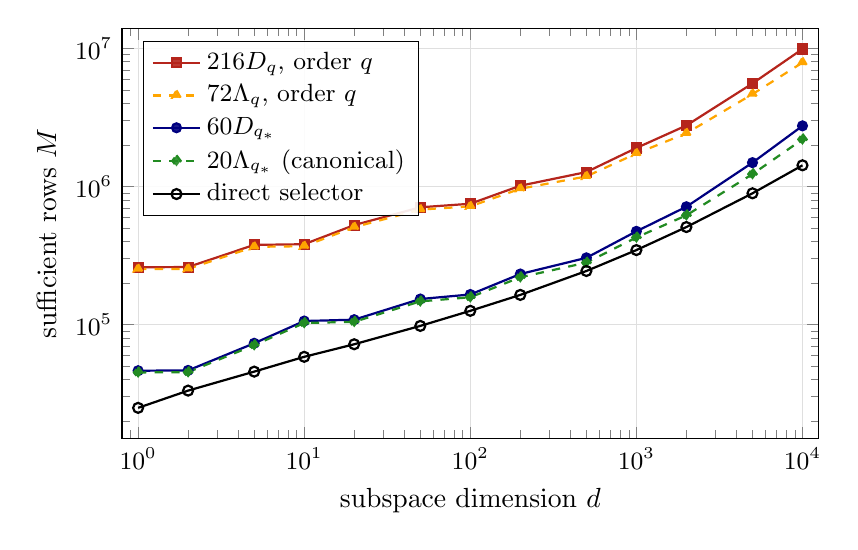
\begin{tikzpicture}
\begin{loglogaxis}[
  width=0.86\textwidth, height=0.56\textwidth,
  xlabel={subspace dimension $d$}, ylabel={sufficient rows $M$},
  xmin=0.8, xmax=12500, ymin=1.5e4, ymax=1.4e7,
  legend pos=north west, legend cell align=left,
  legend style={font=\small,fill=white,fill opacity=0.9,text opacity=1},
  grid=major, grid style={gray!25}, tick label style={font=\small}]
\addplot[thick,BrickRed,mark=square*,mark size=1.6pt] coordinates {
(1,260064)(2,260928)(5,377568)(10,381888)(20,525312)(50,706752)(100,749952)
(200,1012608)(500,1271808)(1000,1900800)(2000,2764800)(5000,5574528)(10000,9894528)};
\addlegendentry{$216D_q$, order $q$}
\addplot[thick,Orange,dashed,mark=triangle*,mark size=1.8pt] coordinates {
(1,252288)(2,253056)(5,365560)(10,369386)(20,507173)(50,680085)(100,717818)
(200,962842)(500,1182839)(1000,1733312)(2000,2428200)(5000,4663626)(10000,7894646)};
\addlegendentry{$72\Lambda_q$, order $q$}
\addplot[thick,NavyBlue,mark=*,mark size=1.6pt] coordinates {
(1,46320)(2,46560)(5,73200)(10,106080)(20,108480)(50,153120)(100,165120)
(200,232320)(500,304320)(1000,473280)(2000,713280)(5000,1488000)(10000,2748480)};
\addlegendentry{$60D_{q_*}$}
\addplot[thick,ForestGreen,dashed,mark=diamond*,mark size=2pt] coordinates {
(1,45012)(2,45226)(5,70933)(10,102608)(20,104728)(50,147210)(100,157664)
(200,220115)(500,280783)(1000,427412)(2000,618440)(5000,1228981)(10000,2192958)};
\addlegendentry{$20\Lambda_{q_*}$ (canonical)}
\addplot[thick,black,mark=o,mark size=1.8pt] coordinates {
(1,24935)(2,33245)(5,45629)(10,58406)(20,72018)(50,97784)(100,125760)
(200,163964)(500,244304)(1000,346325)(2000,508300)(5000,892402)(10000,1423405)};
\addlegendentry{direct selector}
\end{loglogaxis}
\end{tikzpicture}
\caption{Sufficient rows against $d$ ($n=2^{30}$, $\eps=1/2$, $\delta=0.01$,
flat transforms). The steps of the upper curves are jumps of the moment order.
The selector orders are $2,3,3,4,4,5,6,6,8,10,12,15,18$ at the plotted $d$.}
\label{fig:rows}
\end{figure}

\begin{table}[ht]
\centering\small
\begin{tabular}{rrrrrrr}
\toprule
$d$ & $q$ & $q_f$ & $72\Lambda_q$ & $72\Lambda_{q_f}$ & saving & $20\Lambda_{q_*}$\\
\midrule
1 & 5 & 4 & 252\,288 & 162\,041 & 35.8\% & 45\,012\\
10 & 6 & 5 & 369\,386 & 259\,190 & 29.8\% & 102\,608\\
100 & 8 & 7 & 717\,818 & 567\,591 & 20.9\% & 157\,664\\
1\,000 & 10 & 9 & 1\,733\,312 & 1\,538\,681 & 11.2\% & 427\,412\\
10\,000 & 11 & 10 & 7\,894\,646 & 7\,628\,223 & 3.4\% & 2\,192\,958\\
\bottomrule
\end{tabular}
\caption{The reduced order of Corollary~\ref{cor:qf}. Dropping one order in the
crude-root prescription saves up to about a third of the rows at small $d$;
the canonical prescription is smaller still.}
\label{tab:qslack}
\end{table}

\begin{table}[ht]
\centering\small
\begin{tabular}{lrrrrr}
\toprule
Confidence price & $\overline\Gamma$ & $q_*$ & $20\Lambda_{q_*}$ & $60D_{q_*}$ & direct ($q$)\\
\midrule
fixed frame & $1$ & 7 & 157\,664 & 165\,120 & 125\,760 (6)\\
two flat bands, $5+5$ & $252$ & 11 & 357\,798 & 372\,480 & 276\,534 (8)\\
arbitrary spectrum & $10!$ & 18 & 921\,368 & 957\,120 & 696\,744 (12)\\
dictionary union bound & $\binom{1000}{10}\approx2.6\cdot10^{23}$ & 46 & 5\,892\,073 & 6\,118\,080 & 4\,467\,916 (31)\\
\bottomrule
\end{tabular}
\caption{RP-selected frames (Corollary~\ref{cor:gate}) for $d=100$, $k=10$,
$N=1000$. Without any spectral information the factorial gate uses $84\%$
fewer rows than the union bound over the dictionary. The direct column runs
Algorithm~\ref{alg:selector} at confidence $\delta/\overline\Gamma$.}
\label{tab:gate}
\end{table}

\begin{table}[ht]
\centering\small
\begin{tabular}{rrrrr}
\toprule
$d$ & $q_*$ at $\delta/2$ & $20\Lambda_{q_*}$ & $q_*$ at $8\delta^2/9$ & $20\Lambda_{q_*}$\\
\midrule
10 & 6 & 102\,608 & 9 & 227\,705\\
100 & 8 & 199\,394 & 11 & 357\,798\\
1\,000 & 9 & 427\,412 & 12 & 605\,597\\
10\,000 & 11 & 2\,192\,958 & 14 & 2\,442\,162\\
\bottomrule
\end{tabular}
\caption{Rank-two selection (Proposition~\ref{prop:ranktwo}): the pointwise
allowance $\delta/2$ against the second-moment allowance $8\delta^2/9$.}
\label{tab:ranktwo}
\end{table}

\paragraph{Whole-sketch identities (numerical verification).}
We enumerated the complete real flat Walsh laws: at $n=4$ all $2^4\cdot2^4$
sign pairs and all $M$-subsets in exact rational arithmetic, and at $n=8$ in
double precision, for integer PSD test matrices. The identities~\eqref{eq:twoexact},
Theorem~\ref{thm:oneround} and Proposition~\ref{prop:covmap} held exactly at
$n=4$ for $M=1,2,3$ and to $10^{-9}$ at $n=8$. Table~\ref{tab:whole} shows
representative values; the Nystr\"om residual was below the Gram-error energy
and below~\eqref{eq:simple} in every case.

\begin{table}[ht]
\centering\small
\setlength{\tabcolsep}{4pt}
\begin{tabular}{llrrrr}
\toprule
case & law & Gram energy & formula & $\E\norm{K-\Nys_K}_F^2$ & bound~\eqref{eq:simple}\\
\midrule
$n=4$, $M=1$, rank 3 & two-round & 2203.5 & 2203.5 & 556.8 & 4213.5\\
 & one-round & 2738.0 & 2738.0 & 717.2 & 4213.5\\
$n=4$, $M=2$, rank 3 & two-round & 734.5 & 734.5 & 167.1 & 1404.5\\
 & one-round & 912.67 & 912.67 & 280.9 & 1404.5\\
$n=8$, $M=3$, rank 3 & two-round & 2512.32 & 2512.32 & 20.0 & 4250.4\\
 & one-round & 2620.95 & 2620.95 & 2.5 & 4250.4\\
$n=8$, $M=3$, $K=\mathbf 1\mathbf 1^{\mathsf T}/n$ & two-round & 0.3125 & 0.3125 & 0.038 & 0.4167\\
 & one-round & 0.4167 & 0.4167 & 0.070 & 0.4167\\
$n=8$, $M=3$, $K=e_1e_1^{\mathsf T}$ & two-round & 0.4167 & 0.4167 & 0 & 0.4167\\
 & one-round & 0 & 0 & 0 & 0.4167\\
\bottomrule
\end{tabular}
\caption{Exact enumeration of the whole-sketch law (numerical). ``Gram energy''
is $\E\tr[K(G-I)K(G-I)]$ and ``formula'' is~\eqref{eq:twoexact} or
Theorem~\ref{thm:oneround}. The last two
cases show that neither Gram-error energy dominates the other
(Remark~\ref{rem:blind}); the rank-three rows show how far the rank-blind bound
is from the true Nystr\"om residual.}
\label{tab:whole}
\end{table}

\paragraph{Scalar checks.} $2/\sqrt{20}+1/20=0.49721$, $\sqrt2/3+1/36=0.49918$,
$12/\sqrt{646}+18/646=0.4999975$, $\sqrt\pi/24=0.07385<1/12$. The atom bound of
Lemma~\ref{lem:atom} was checked for all $2\le n\le400$, $1\le M<n$ (maximal
ratio of atom to bound $1$, attained at $n=2$, $M=1$ where both equal $1/2$).
On a grid of coherences $\alpha\in[1,10]$, $\beta\in[1,5]$, $q\le30$, the ratio
$\Lambda_q/D_q$ ranged over $[2.07,3.00)$. Numerically
$g(1+\beta)^{1/\beta}=2.08402$, $2.07442$, $2.0743278$ at $\beta=10^{-2},10^{-4},10^{-8}$.
For sketched RP (Proposition~\ref{prop:pathlocal}) at $\eps_0=1/8$ and $q=\ell$ the
row counts are $1.36\cdot10^6$, $2.89\cdot10^7$ and $1.13\cdot10^8$ for
$\ell=11,51,101$.

%======================================================================
\FloatBarrier
\section{Open problems}\label{sec:open}

\begin{enumerate}[label=\arabic*.]
\item \emph{The confidence term.} All prescriptions keep the allowance
$d+12q^2$ with $q\asymp\log(d/\delta)$. The support-alignment example
of~\cite{SRHT2R,V11} rules out a uniform $d+\log(1/\delta)$ term for any fixed
number of transform-sign layers, but the gap between $\log^2$ and the
obstruction is open, as is the constant $12$.
\item \emph{Efficient search of the certified widths.}
The uncapped root is globally nonmonotone, as Remark~\ref{rem:selector}
shows. Determine whether its feasible set has a monotone structure in
the useful regime, or use the stronger imported allowance
$L_q\le\min\{1,\Lambda_q/n\}$ to obtain a search guarantee.
A proof is needed before bisection can be asserted to return a global
minimum.
\item \emph{A tail-relative high-probability whole-sketch bound.}
Theorem~\ref{thm:whole} is rank-blind, and the finite-support obstruction
of Remark~\ref{rem:blind} rules out a uniform expected bound depending
only on a spectral tail when $M<n$. Determine a high-probability relative
trace or Frobenius bound for one two-round sketch with shared signs,
with explicit dependence on rank, distortion and failure probability.
\item \emph{Rows linear in the pivot budget.} The hybrid path comparison
in~\cite{RobustRP} already reduces the order to
$O(\eta^2k+\log(k\tr A/(\eps\tau)))$, but the certified two-round SRHT
budget remains quadratic in $k$ at fixed distortion. Can a sharper
embedding or path comparison yield a budget linear in $k$?
\item \emph{Beyond the fixed-range gate.} The gate needs full rank, a fixed range and
an unordered release. A price for partial-rank or moving-range selection would
cover the natural pipeline in which the frame is the span of the first pivots.
\item \emph{Block drift.} The whole-block mixed moment of the real flat law suggests a
drift constant $1+\frac2M(1-\frac Mn)$ for a full block of $M$ shared rows. A
proof with explicit dependence on the shared signs would connect
Theorem~\ref{thm:drift} and Theorem~\ref{thm:whole}.
\end{enumerate}

%======================================================================
\begin{thebibliography}{99}\small\raggedright

\bibitem{AilonChazelle}
N.~Ailon and B.~Chazelle.
\newblock The fast Johnson--Lindenstrauss transform and approximate nearest neighbors.
\newblock \emph{SIAM J. Comput.} 39(1):302--322, 2009.

\newblock \url{https://doi.org/10.1137/060673096}
\newblock Author copy: \url{https://www.cs.princeton.edu/~chazelle/pubs/FJLT-sicomp09.pdf}

\bibitem{Amsel}
N.~Amsel et al.
\newblock Linear systems and eigenvalue problems: open questions from a Simons workshop.
\newblock arXiv:2602.05394, 2026. Definition~5.3 and Problem~5.6.

\newblock \url{https://arxiv.org/abs/2602.05394v3}

\bibitem{BBGL}
O.~Balabanov, M.~Beaup\`ere, L.~Grigori and V.~Lederer.
\newblock Block subsampled randomized Hadamard transform for Nystr\"om approximation on distributed architectures.
\newblock \emph{Proc. ICML}, PMLR 202:1564--1576, 2023.

\newblock \url{https://proceedings.mlr.press/v202/balabanov23a.html}

\bibitem{BN}
R.~A.~Baston and Y.~Nakatsukasa.
\newblock Stochastic diagonal estimation: probabilistic bounds and an improved algorithm.
\newblock arXiv:2201.10684, 2022.

\newblock \url{https://arxiv.org/abs/2201.10684}

\bibitem{BoutsidisGittens}
C.~Boutsidis and A.~Gittens.
\newblock Improved matrix algorithms via the subsampled randomized Hadamard transform.
\newblock \emph{SIAM J. Matrix Anal. Appl.} 34(3):1301--1340, 2013. arXiv:1204.0062.

\newblock \url{https://arxiv.org/abs/1204.0062}

\bibitem{CEMT}
C.~Cama\~no, E.~N.~Epperly, R.~A.~Meyer and J.~A.~Tropp.
\newblock Faster linear algebra algorithms with structured random matrices.
\newblock arXiv:2508.21189, 2025.

\newblock \url{https://arxiv.org/abs/2508.21189}

\bibitem{CETW}
Y.~Chen, E.~N.~Epperly, J.~A.~Tropp and R.~J.~Webber.
\newblock Randomly pivoted Cholesky: practical approximation of a kernel matrix with few entry evaluations.
\newblock \emph{Comm. Pure Appl. Math.}, 2025. arXiv:2207.06503.

\newblock \url{https://arxiv.org/abs/2207.06503}

\bibitem{DV}
A.~Deshpande and S.~Vempala.
\newblock Adaptive sampling and fast low-rank matrix approximation.
\newblock In \emph{APPROX/RANDOM 2006}, LNCS 4110, 292--303, 2006. ECCC report TR06-042, Proposition~7.

\newblock \url{https://eccc.weizmann.ac.il/report/2006/042/}

\bibitem{DRVW}
A.~Deshpande, L.~Rademacher, S.~Vempala and G.~Wang.
\newblock Matrix approximation and projective clustering via volume sampling.
\newblock \emph{Theory of Computing} 2:225--247, 2006.

\newblock \url{https://theoryofcomputing.org/articles/v002a012/}

\bibitem{DKM}
P.~Drineas, R.~Kannan and M.~W.~Mahoney.
\newblock Fast Monte Carlo algorithms for matrices I: approximating matrix multiplication.
\newblock \emph{SIAM J. Comput.} 36(1):132--157, 2006.

\newblock \url{https://doi.org/10.1137/S0097539704442684}
\newblock Author copy: \url{https://www.cs.yale.edu/homes/mmahoney/pubs/matrix1_SICOMP.pdf}

\bibitem{DMMS}
P.~Drineas, M.~W.~Mahoney, S.~Muthukrishnan and T.~Sarl\'os.
\newblock Faster least squares approximation.
\newblock \emph{Numer. Math.} 117:219--249, 2011. arXiv:0710.1435.

\newblock \url{https://arxiv.org/abs/0710.1435}

\bibitem{GrossNesme}
D.~Gross and V.~Nesme.
\newblock Note on sampling without replacing from a finite collection of matrices.
\newblock arXiv:1001.2738, 2010.

\newblock \url{https://arxiv.org/abs/1001.2738v2}

\bibitem{Haagerup}
U.~Haagerup.
\newblock The best constants in the Khintchine inequality.
\newblock \emph{Studia Math.} 70(3):231--283, 1981.

\newblock \url{https://doi.org/10.4064/sm-70-3-231-283}

\bibitem{HY}
D.~Heidary.
\newblock \emph{Two-round SRHT: hybrid constants and proof-chain comparison.}
\newblock Repository manuscript, September 2026.

\newblock \url{https://github.com/DiarHaidary/Results/blob/main/Wick-Hermite%20Hybrid/srht_hybrid_constants_template.pdf}

\bibitem{V11}
D.~Heidary.
\newblock \emph{Graded Multiplication Operators for Random-Matrix Moments.}
\newblock Repository manuscript, September 2026.

\newblock \url{https://github.com/DiarHaidary/Results/blob/main/Graded%20Multiplication%20Operators%20for%20Random-Matrix%20Moments.pdf}

\bibitem{SRHT2R}
D.~Heidary.
\newblock \emph{Two-round Walsh transforms as subspace embeddings.}
\newblock Repository manuscript, September 2026.

\newblock \url{https://github.com/DiarHaidary/Results/blob/main/SRHT.pdf}

\bibitem{RA01}
D.~Heidary.
\newblock \emph{Iterated-logarithmic pivot bounds for randomly pivoted Cholesky.}
\newblock Repository manuscript, September 2026.

\newblock \url{https://github.com/DiarHaidary/Results/blob/main/manuscripts/background/Iterated_Logarithmic_RPCholesky.pdf}

\bibitem{RobustRP}
D.~Heidary.
\newblock \emph{RPCholesky under approximate and sketched pivot probabilities.}
\newblock Repository manuscript, September 2026.

\newblock \url{https://github.com/DiarHaidary/Results/blob/main/manuscripts/06-Robust-Sketched-RPCholesky/RPCholesky_Approximate_Sketched_Pivots.pdf}

\bibitem{PP}
D.~Heidary.
\newblock \emph{Product-Probe Drift, Kronecker Nystr\"om Approximation, and Trace Estimation.}
\newblock Repository manuscript, September 2026.

\newblock \url{https://github.com/DiarHaidary/Results/blob/main/manuscripts/02-Product-Probe-Drift/Product_Probe_Drift_v2.pdf}

\bibitem{SparseStack}
D.~Heidary.
\newblock \emph{SparseStack Is an Optimal Oblivious Subspace Embedding.}
\newblock Repository manuscript, September 2026.

\newblock \url{https://github.com/DiarHaidary/Results/blob/main/SparseStack.pdf}

\bibitem{Hutchpp}
R.~A.~Meyer, C.~Musco, C.~Musco and D.~P.~Woodruff.
\newblock Hutch++: optimal stochastic trace estimation.
\newblock In \emph{Proc. SOSA}, 142--155, 2021. arXiv:2010.09649.

\newblock \url{https://arxiv.org/abs/2010.09649}

\bibitem{Mordhorst}
O.~Mordhorst.
\newblock The optimal constants in Khintchine's inequality for the case $2<p<3$.
\newblock \emph{Colloq. Math.} 147(2):203--216, 2017. arXiv:1601.07850.

\newblock \url{https://arxiv.org/abs/1601.07850}

\bibitem{TroppSRHT}
J.~A.~Tropp.
\newblock Improved analysis of the subsampled randomized Hadamard transform.
\newblock \emph{Adv. Adapt. Data Anal.} 3(1--2):115--126, 2011. arXiv:1011.1595.

\newblock \url{https://arxiv.org/abs/1011.1595}

\bibitem{Yang}
Y.~Yang.
\newblock Subspace embeddings with the rerandomized SRHT.
\newblock arXiv:2609.13946v1, September 2026, Theorem~1.
\newblock \url{https://arxiv.org/abs/2609.13946v1}
\newblock \url{https://github.com/yuningyang19/OpenProblemsInNLA_TR-01/blob/ed21181197ac839eac95f549404f94e7e3aa6e10/manuscript.pdf}

\bibitem{SparseCompanion}
D.~Heidary.
\newblock \emph{SparseStack: sampling prescriptions and adaptive frames.}
\newblock Repository companion manuscript, September 2026.
\newblock \url{https://github.com/DiarHaidary/Results/blob/main/manuscripts/04-SparseStack-Companion/SparseStack_Constants_Nystrom_Adaptive.pdf}

\bibitem{Nystrompp}
D.~Persson, A.~Cortinovis and D.~Kressner.
\newblock Improved variants of the Hutch++ algorithm for trace estimation.
\newblock \emph{SIAM J. Matrix Anal. Appl.} 43(3):1162--1185, 2022.
\newblock \url{https://arxiv.org/abs/2109.10659}

\end{thebibliography}
\end{document}
